\documentclass[9pt,a4paper]{report}
\usepackage{mwe}
\usepackage{listings}
\usepackage{amsmath}
\usepackage{graphicx}
\usepackage{subfig}
\usepackage{float}
\usepackage{xcolor}
\usepackage{multirow}
\usepackage{hyperref}
\usepackage{fancyhdr}
\usepackage{sectsty}
\usepackage[dvipsnames]{xcolor}
\usepackage{soul}
\usepackage[compact]{titlesec}
\usepackage{float}
\usepackage[left=0.5cm,right=0.5cm,top=0.5cm,bottom=0.5cm]{geometry}
\graphicspath{{Report/Part 1.1}{Report/Part 1.1/Series Forward-Bias Diode Circuit}{Report/Part 1.2}{Report/Part 1.2/Series Reverse-breakdown Zener Diode Circuit}{Report/Part 1.3}{Report/Part 1.3/Parallel Opposing Polarities Diode Circuit}{Report/Part 1.3/Series Opposing Polarities Zener Diode Circuit}{Report/Part 1.4}{Report/Part 1.4/Full Rectifier circuits/Bridge With Filter}{Report/Part 1.4/Full Rectifier circuits/Bridge With Zener}{Report/Part 1.4/Full Rectifier circuits/Full Wave Bridge}}

\newcommand*{\nchapter}[1]{%
	\chapter*{#1}%
	\addcontentsline{toc}{chapter}{#1}
	\vspace{-14mm}}
\newcommand*{\nsection}[1]{%
	\section*{#1}%
	\addcontentsline{toc}{section}{#1}}
\newcommand*{\nsubsection}[1]{%
	\subsection*{#1}%
	\addcontentsline{toc}{subsection}{#1}}
\newcommand*{\nsubsubsection}[1]{%
	\subsubsection*{#1}%
	\addcontentsline{toc}{subsubsection}{#1}}

\chaptertitlefont{\large}
\sectionfont{\normalsize}
\fontsize{9}{11}\selectfont
\begin{document}
	\begin{titlepage}
		\centering
		\vspace*{1.5in}
		
\includegraphics[width=0.15\textwidth]{W-Logo_Purple_RGB}\par\vspace{1cm}
		{\LARGE \textsc{University of Washington}\par}
		\vspace{1cm}
		{\Large \textsc{BEE331 Lab 1.1}\par}
		\vspace{1.5cm}
		{\huge\bfseries \par}
		\vspace{2cm}
		{\Large\itshape 2301991\hspace{55pt}1900585\par}
		{\Large\itshape Jason Truong\hspace{31pt}Henry Haight\par}
		\vfill
		supervised by\par
		Prof.~Joseph \textsc{Decuir}
		\date{2024\\ January}
		\vfill
		% Bottom of the page
		{\large \today\par}
		\vspace*{1.5in}
	\end{titlepage}
	
	\nchapter{Characterising Diodes; I-V Curve}
	\nsection{Design Objective}
	In this lab, we introduce ourselves to the diode, we characterise its function by the I-V curve.
	\begingroup
	\renewcommand{\cleardoublepage}{}
	\renewcommand{\clearpage}{}
	\nsection{Circuit Design Outline}
	\endgroup
	With a resistor of an arbitrary impedance greater than $100\Omega$ ($R\geq100\Omega$), and the natural impedance of the Function Generator in series ($R_{TOT}=R_{FG}+R\geq150\Omega$), the (1N4148 silicon) diode is set in series to forward-bias from the function generator. Set the function generator @ f=1kHz and $V_P=5V$.
	\begin{figure}[hp!]
		\centering
		\caption{\centering Series R + Diode}
		\subfloat[\centering LTSpice + Rudimentary Schematic Series RD ($499\Omega$) Circuit]{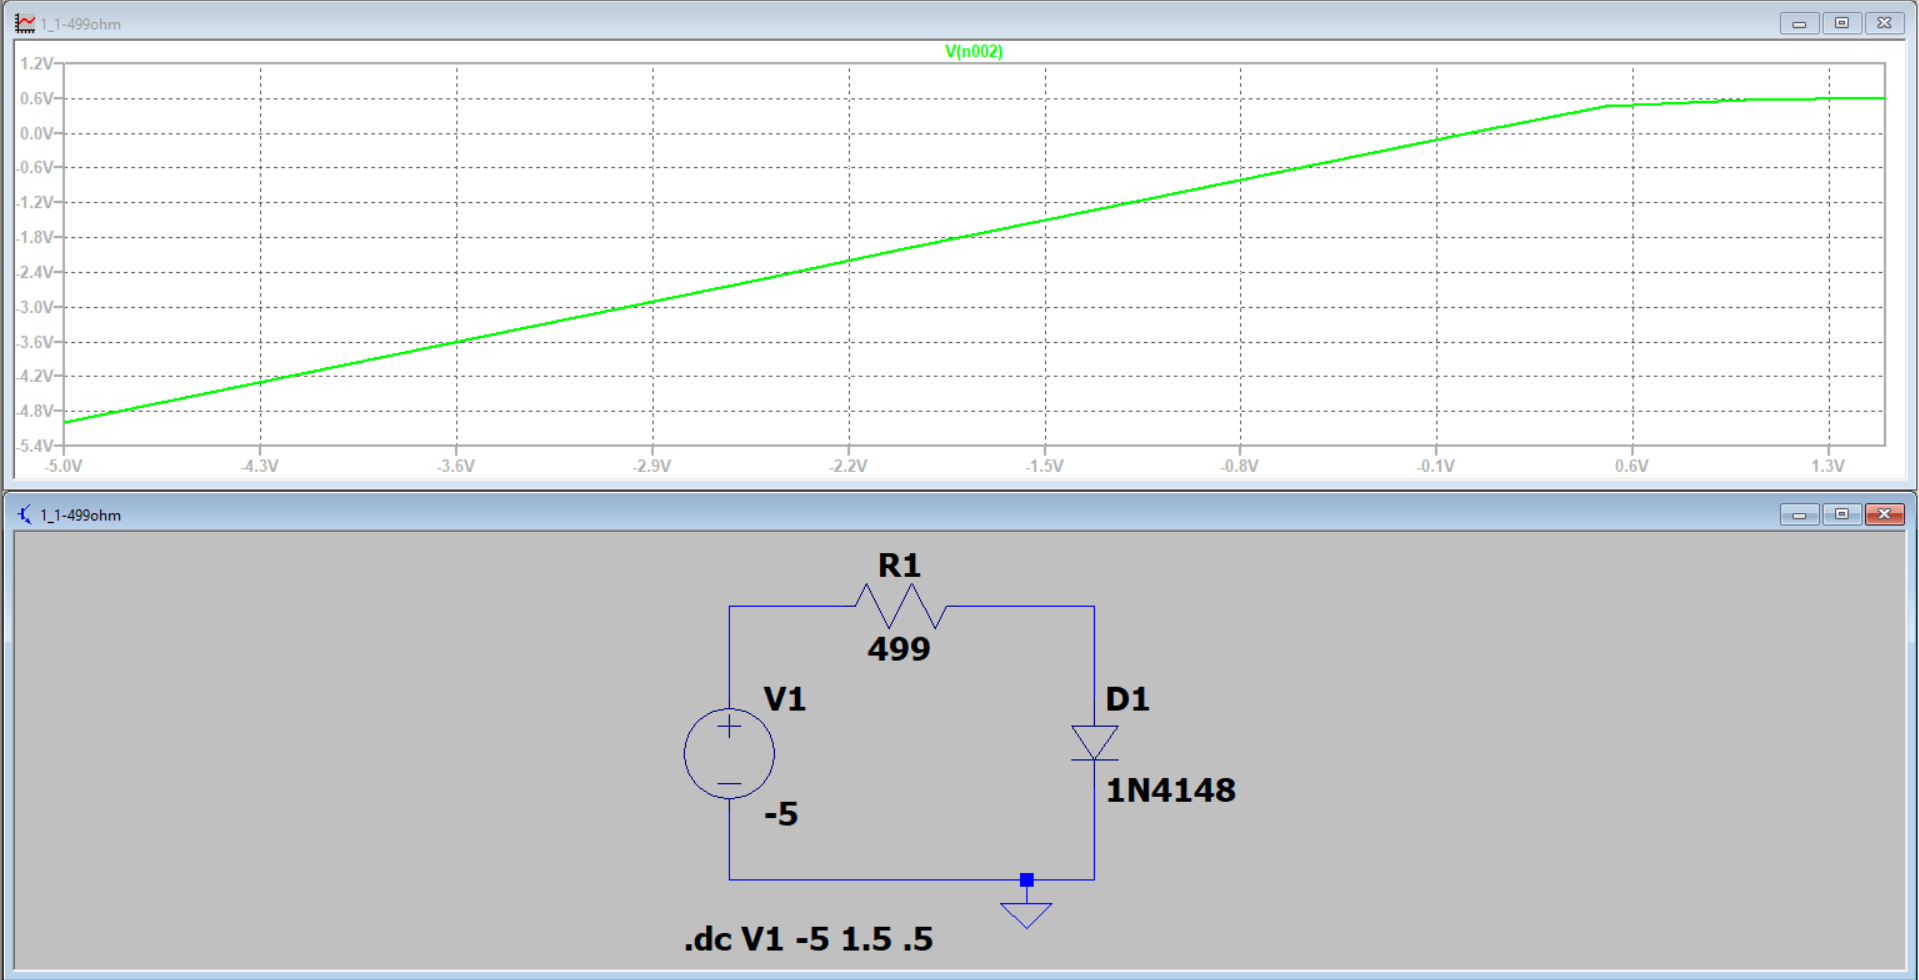
\includegraphics[width=9cm]{499 resistor circuit sim}}\hfil
		\subfloat[\centering LTSpice + Rudimentary Schematic Series RD ($100\Omega$) Circuit]{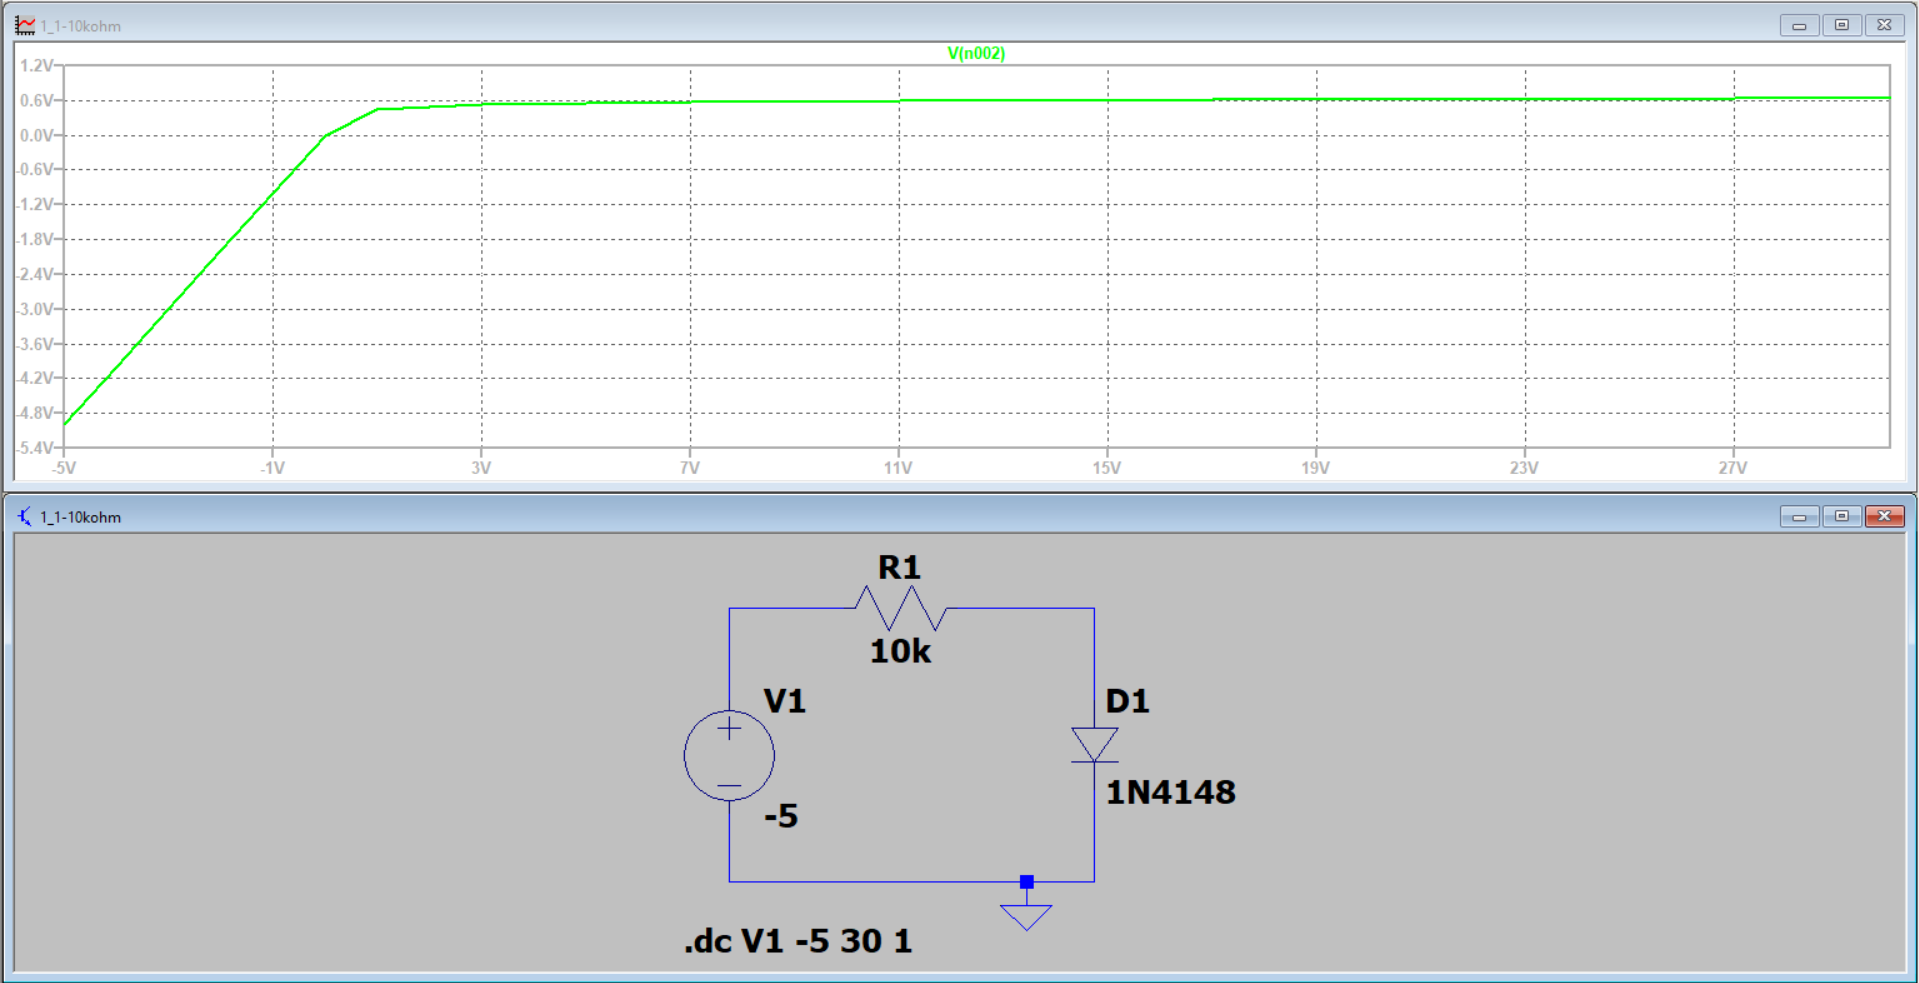
\includegraphics[width=9cm]{100 resistor circuit sim}}
	\end{figure}
	\begin{figure}[hp!]
		\ContinuedFloat
		\centering
		\subfloat[\centering Series RD Circuit $499\Omega$]{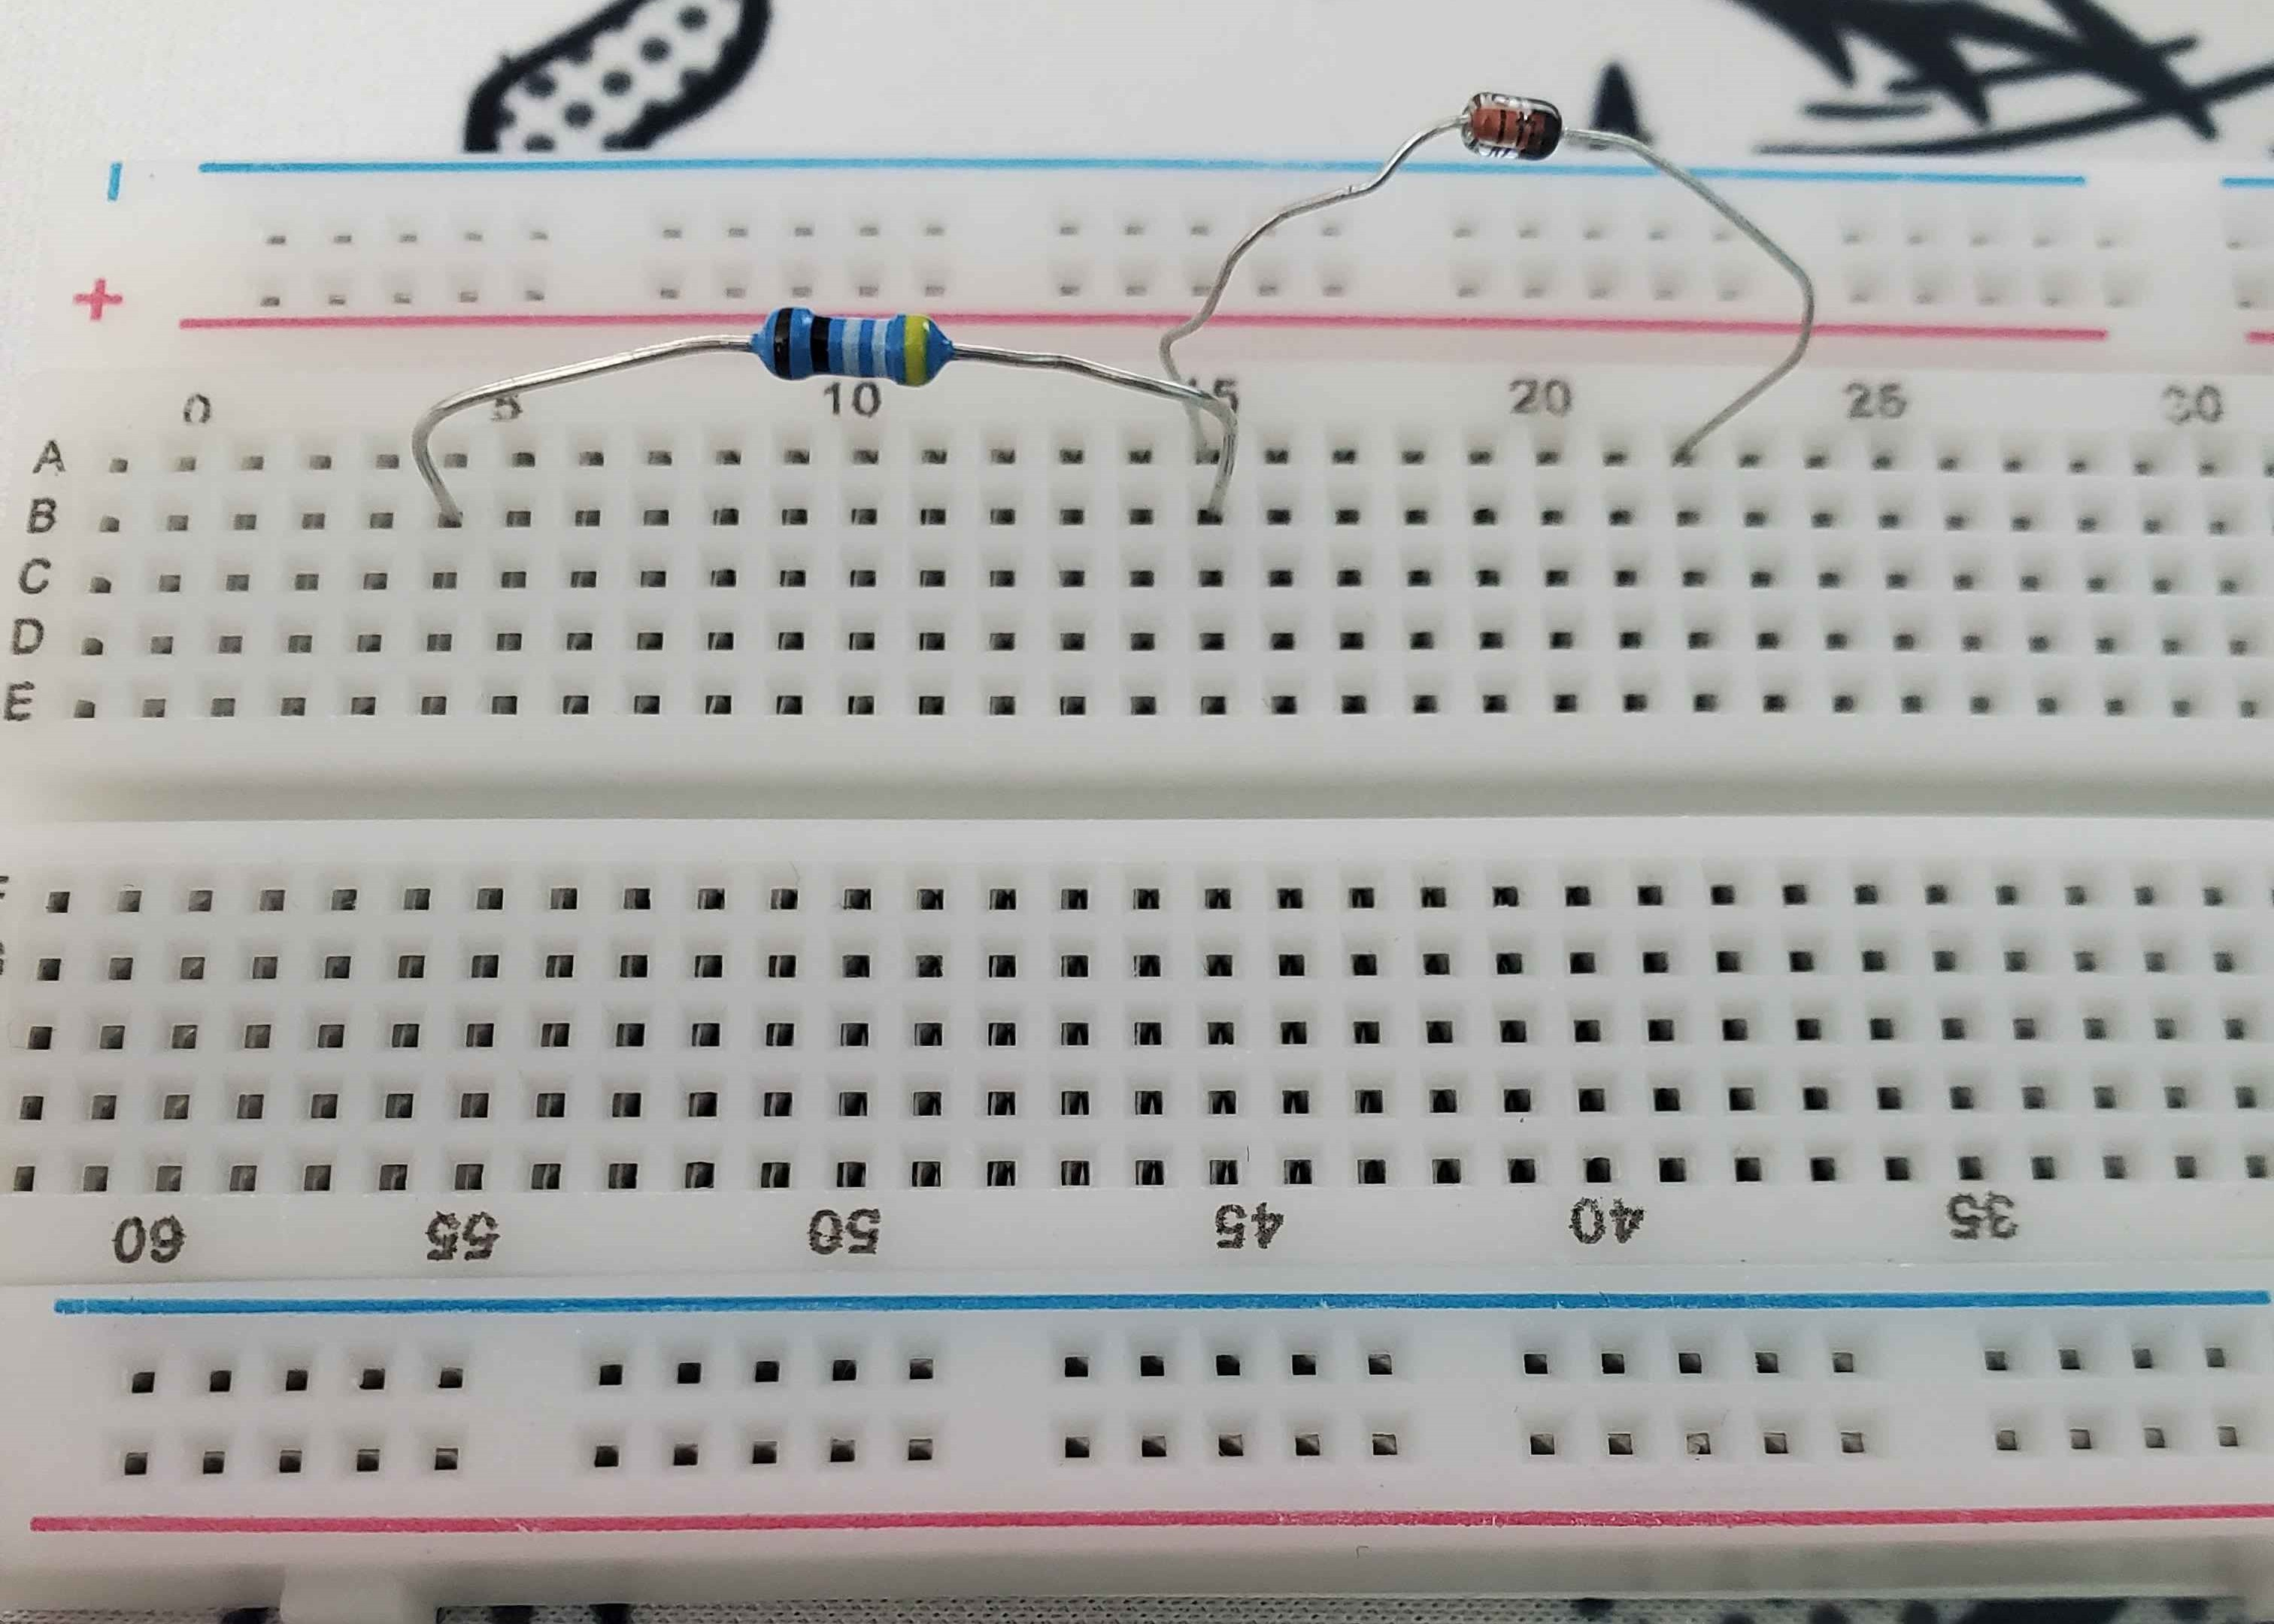
\includegraphics[width=9cm]{499 resistor circuit irl}}\hfil
		\subfloat[\centering Series RD Circuit $100\Omega$]{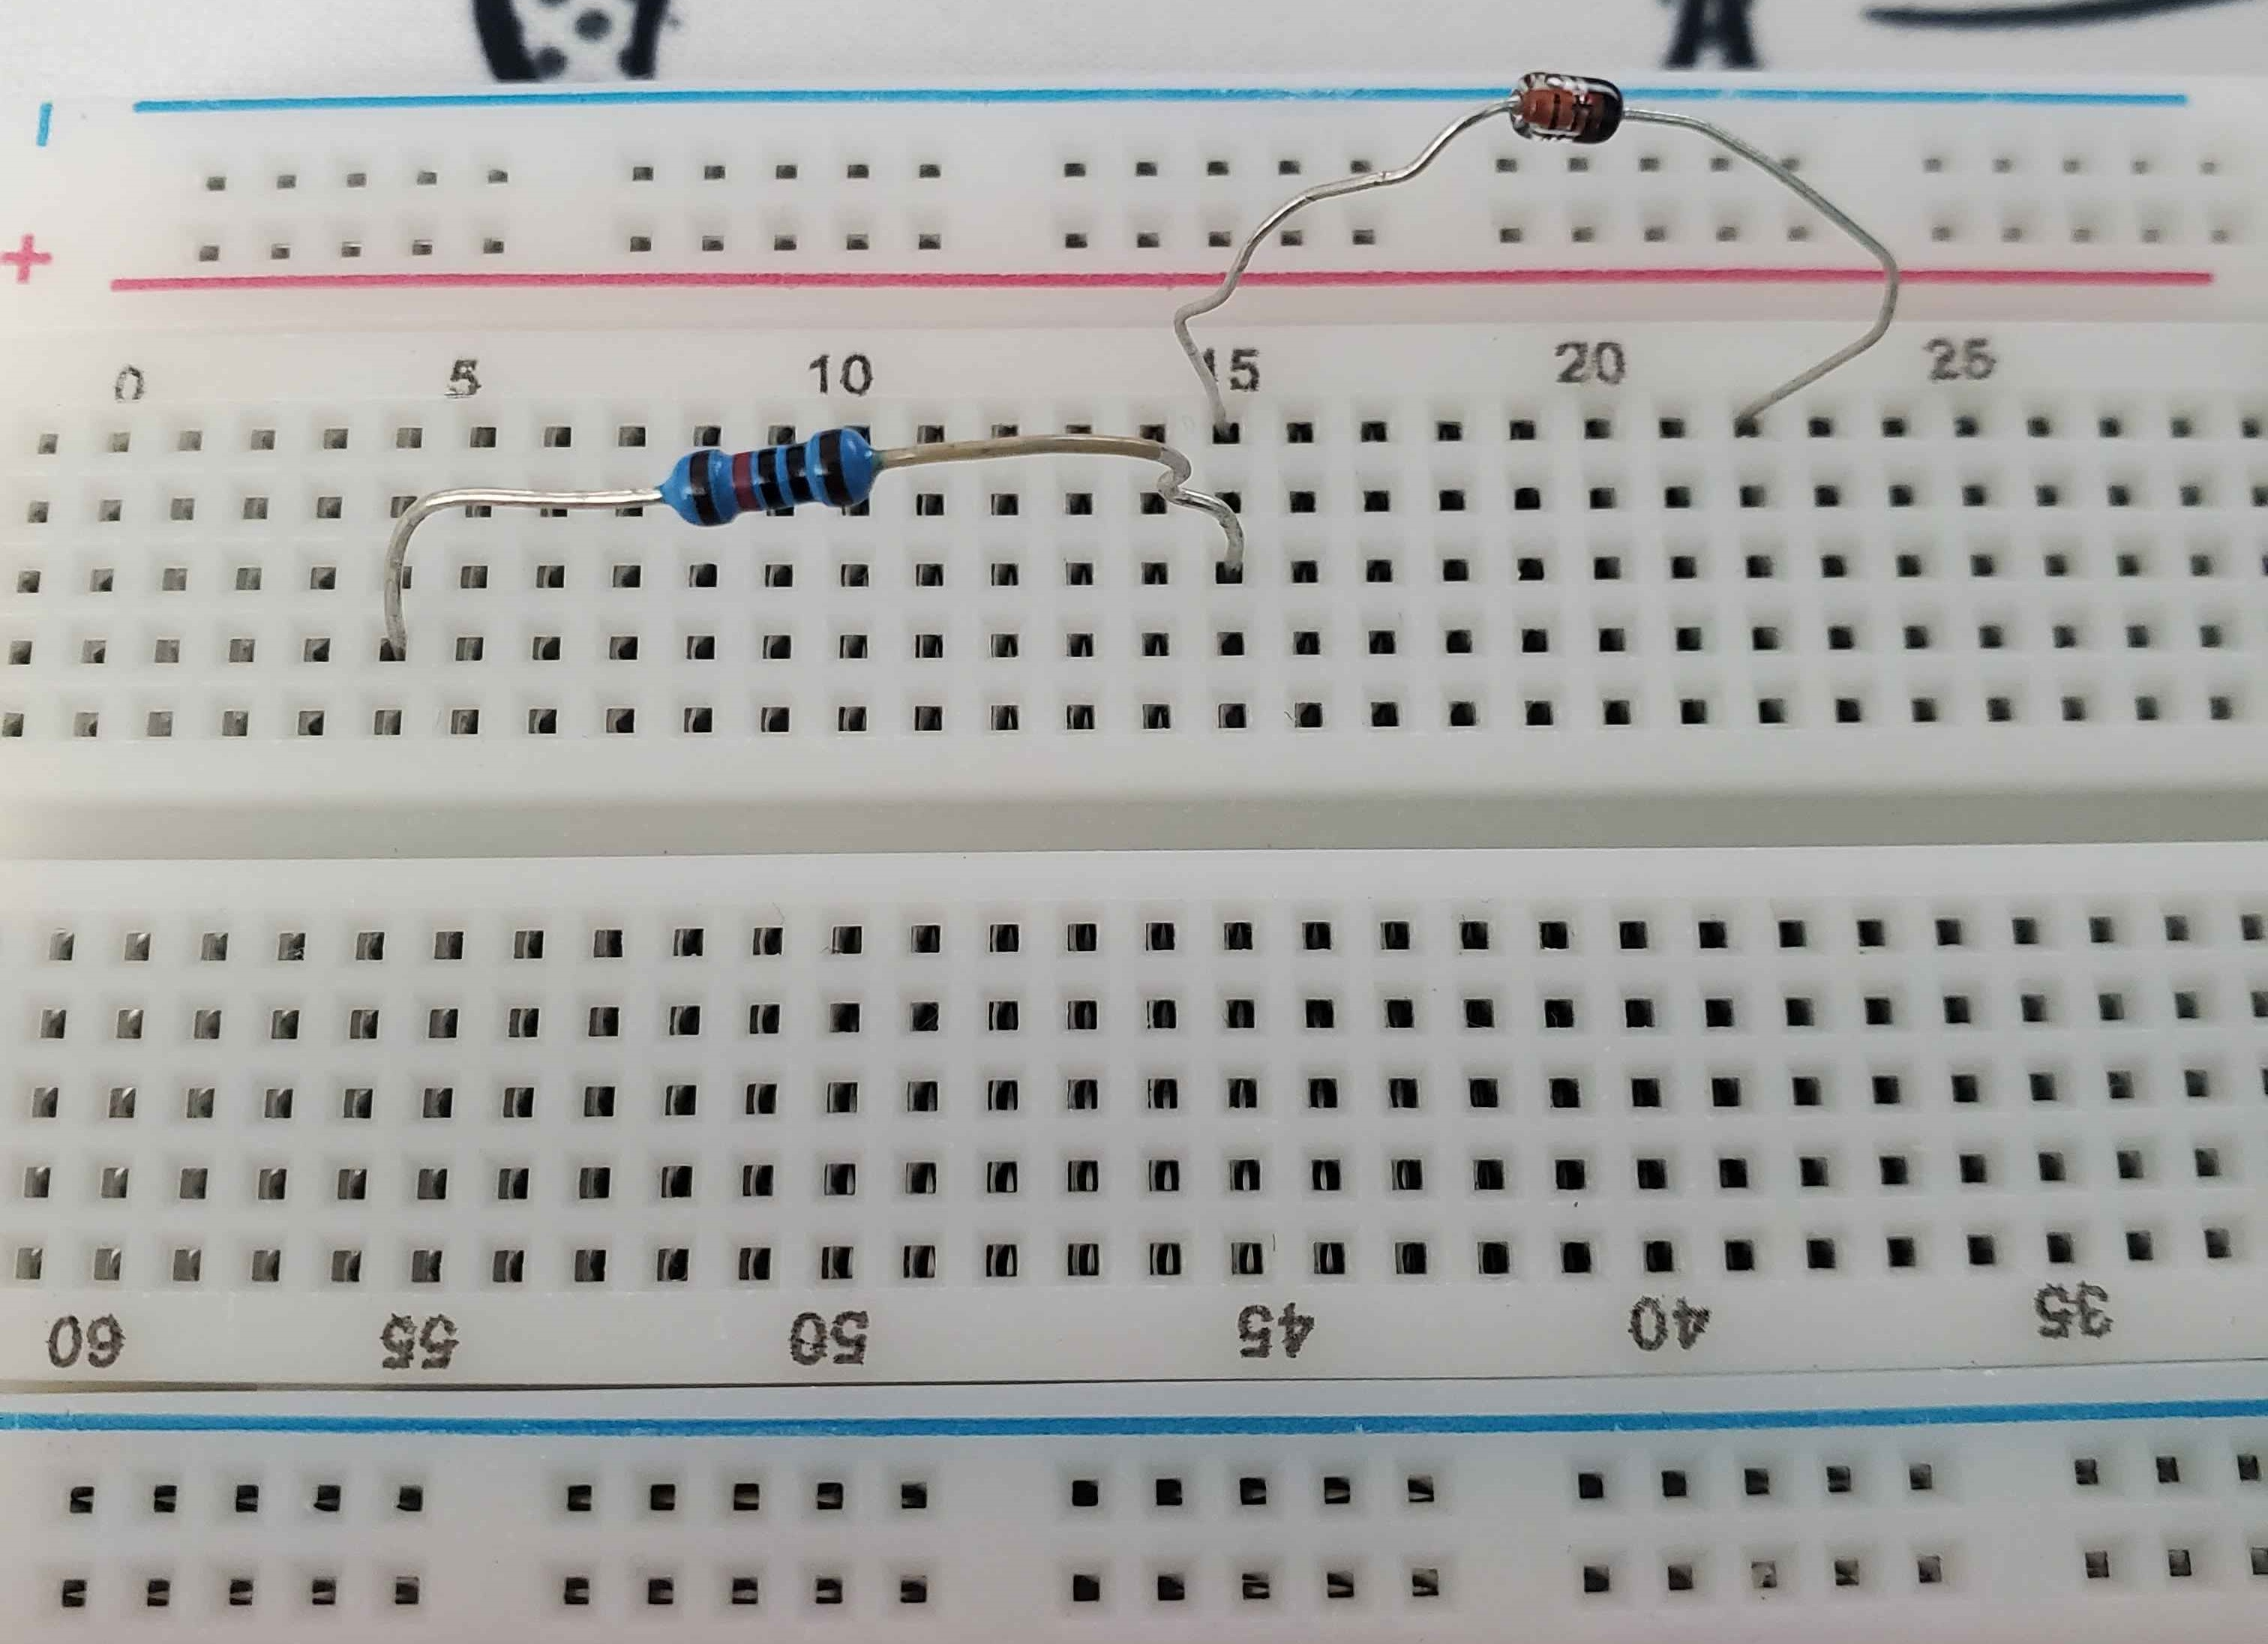
\includegraphics[width=9cm]{100 resistor circuit irl}}
	\end{figure}
	\newpage
	\nsection{Descriptions of Measurements \& Calculations}
	\nsubsection{Analysis}
	\begin{itemize}
		\item \textbf{i. Describe how you measured $I_D$ and $V_D$?}
		\subitem At the node where R; ($R>100\Omega$) and the Diode; ($D$) meet, we denote this junction as $V_{out}$. We attach our Multimetre's positive lead (Red) to $V_{out}$, and attached our ground lead to the opposing node of the Diode; ($D$) - which should be grounded.
		\item \textbf{ii. In this experiment how would you determine the value of $I_{D,max}$}
		\subitem $I_D=I_S(e^{\frac{V_D}{V_T}}-1)$; reference Figure 1b.
		\item \textbf{iii. In the circuit, what limits $I_D$?}
		\subitem The characteristics of the I-V curve of a diode has current $I_D$ exponentially rise towards a cut-off at the threshold, towards the C.V.D @ $V_D$.
		\item \textbf{iv. Explain why $V_D$ does not change much while $I_D$ can change a lot.}
		\subitem Given the equation of a Diode's characteristics of $I_D=I_S(e^{\frac{V_D}{V_T}}-1)$. Putting the equation in reference to $I_D$ is an exponential function, while $V_D$ is a logarithmic function with a very slow rise time.
	\end{itemize}
	\begin{figure}[hp!] %140, 
		\centering
		\caption{RD Circuit}
		\subfloat[RD Circuit Measurement]{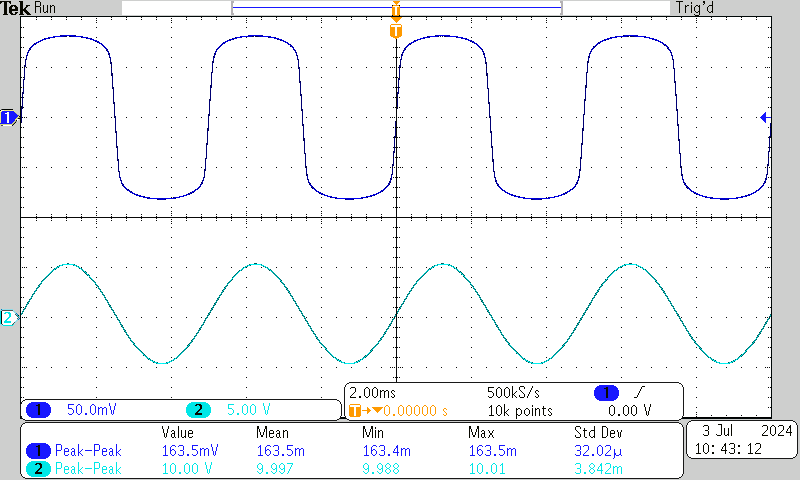
\includegraphics[width=9cm]{tek0001}}
		\subfloat[Sample Measurement ]{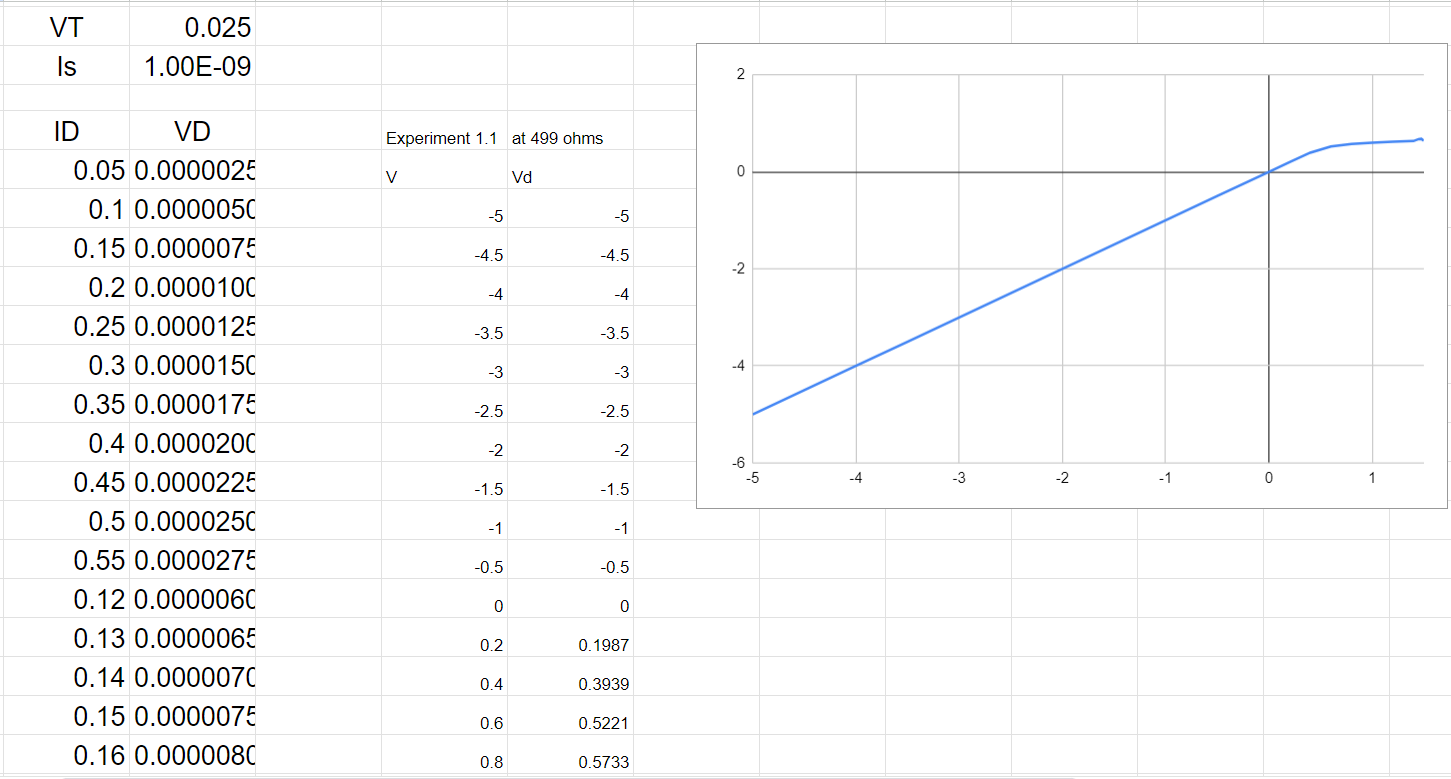
\includegraphics[width=9cm]{Screenshot 2024-07-15 074336}}
	\end{figure}
	\nsection{Summary \& Conclusions}
	Revealed in Figure RD-Circuit 1A \& 1B, the generated oscilloscope readings of the two periodic function match the characteristics of the transfer function found in  1b (RD Circuit). So the measurements do infact closely align.
	
	\nchapter{Characterising Zener Diodes; I-V Curve}
	\nsection{Design Objective}
	In this lab, we introduce ourselves to the \emph{Zener} diode, we characterise its function by the I-V curve.
	\begingroup
	\renewcommand{\cleardoublepage}{}
	\renewcommand{\clearpage}{}
	\nsection{Circuit Design Outline}
	\endgroup
	With a resistor of an arbitrary impedance greater than $100\Omega$ ($R\geq100\Omega$), and the natural impedance of the Function Generator in series ($R_{TOT}=R_{FG}+R\geq150\Omega$), the (1N4732 or 1n5223) Zener diode is set in series set in reverse-polarity to procate reverse-breakdown from the diode; through the function generator. Set the function generator @ f=1kHz and $V_P=5V$ (We'll be focusing on the negative portion of $V_P$).
	\begin{figure}[hp!]
		\centering
		\caption{\centering Series $R$ + Diode $D_Z$}
		\subfloat[\centering LTSpice + Rudimentary Schematic Series RD ($499\Omega$) Circuit]{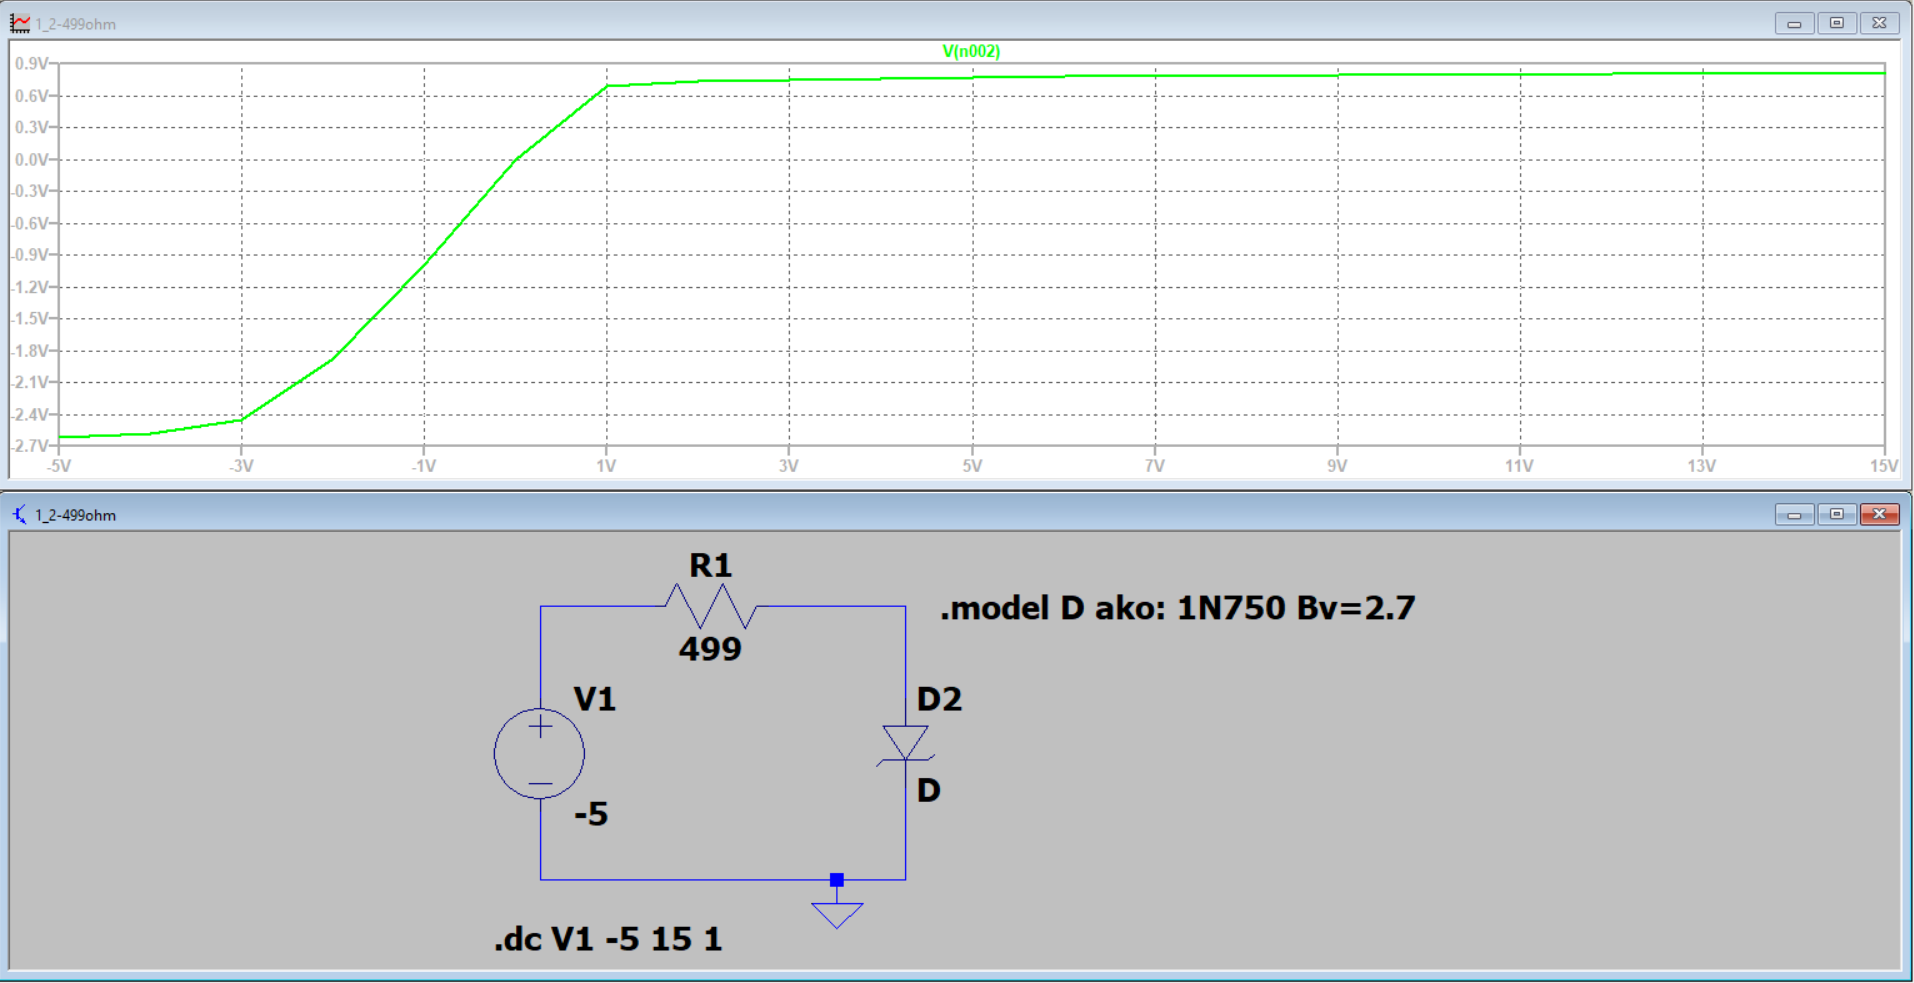
\includegraphics[width=9cm]{Screenshot 2024-07-15 063312}}
		\subfloat[\centering LTSpice + Rudimentary Schematic Series RD ($10k\Omega$) Circuit]{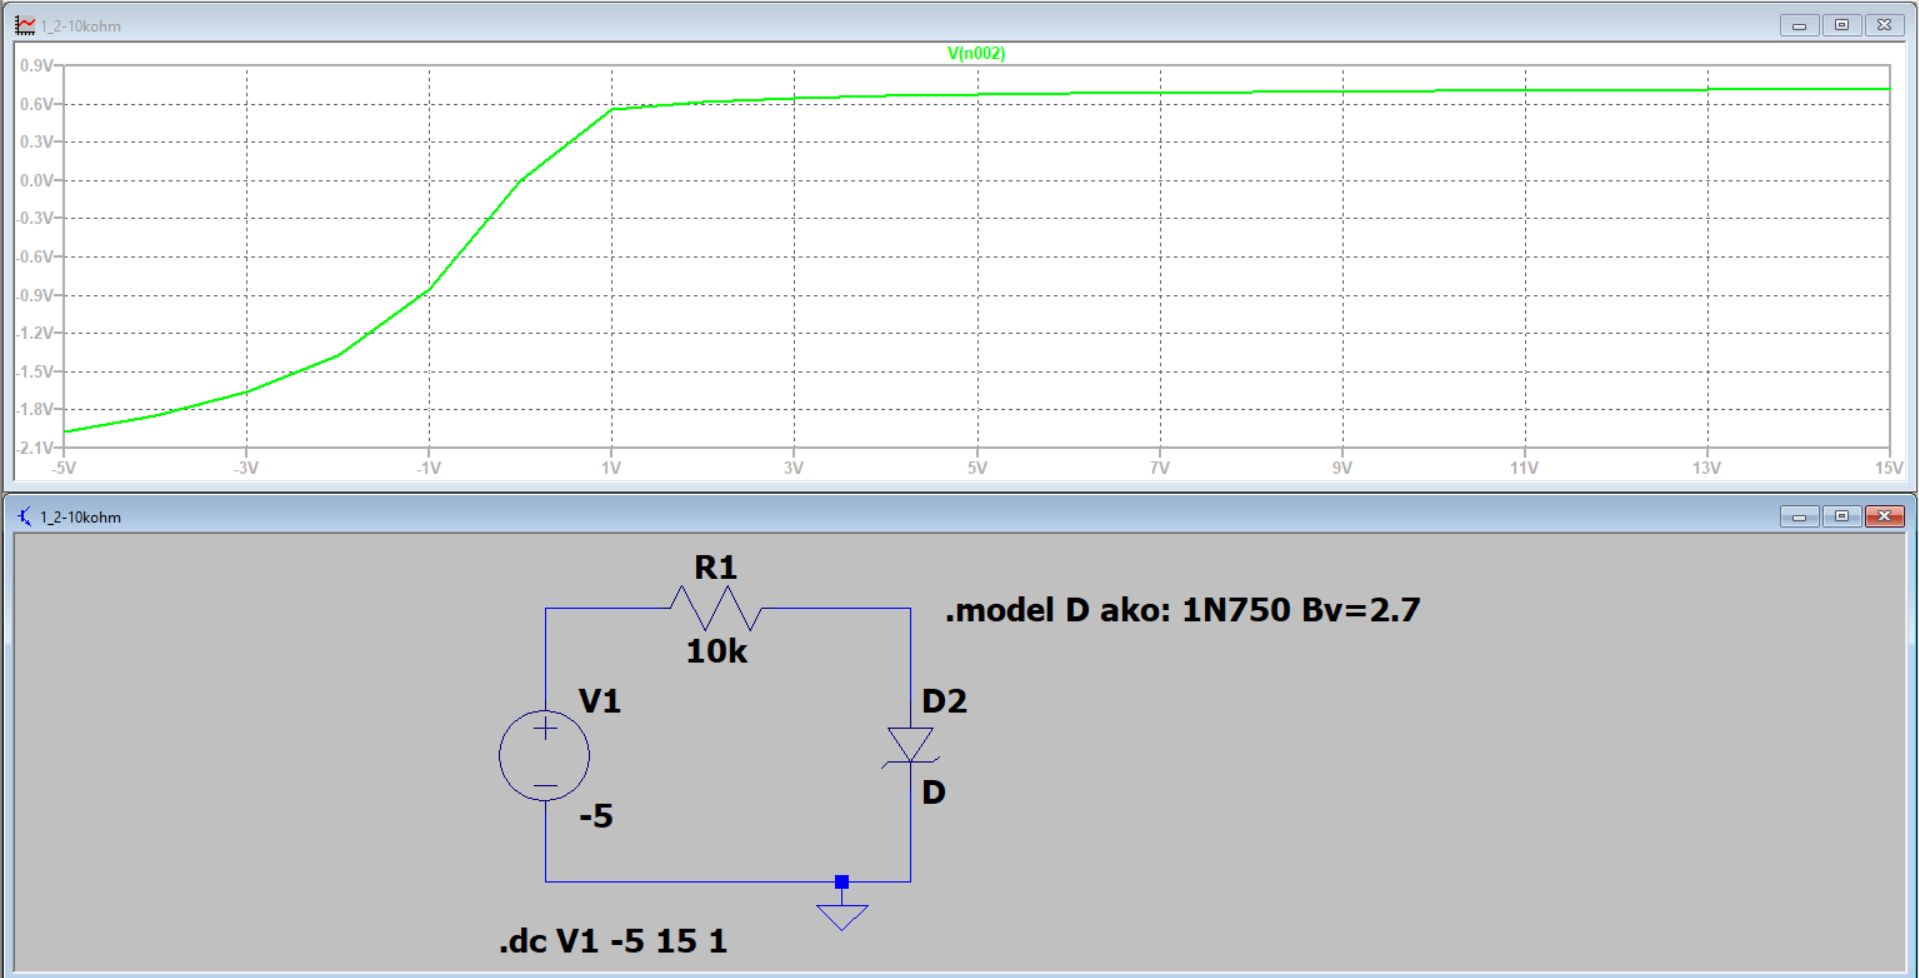
\includegraphics[width=9cm]{Screenshot 2024-07-15 062954}}
	\end{figure}
	\begin{figure}[hp!]
		\ContinuedFloat
		\centering
		\subfloat[\centering Series RD Circuit $499\Omega$]{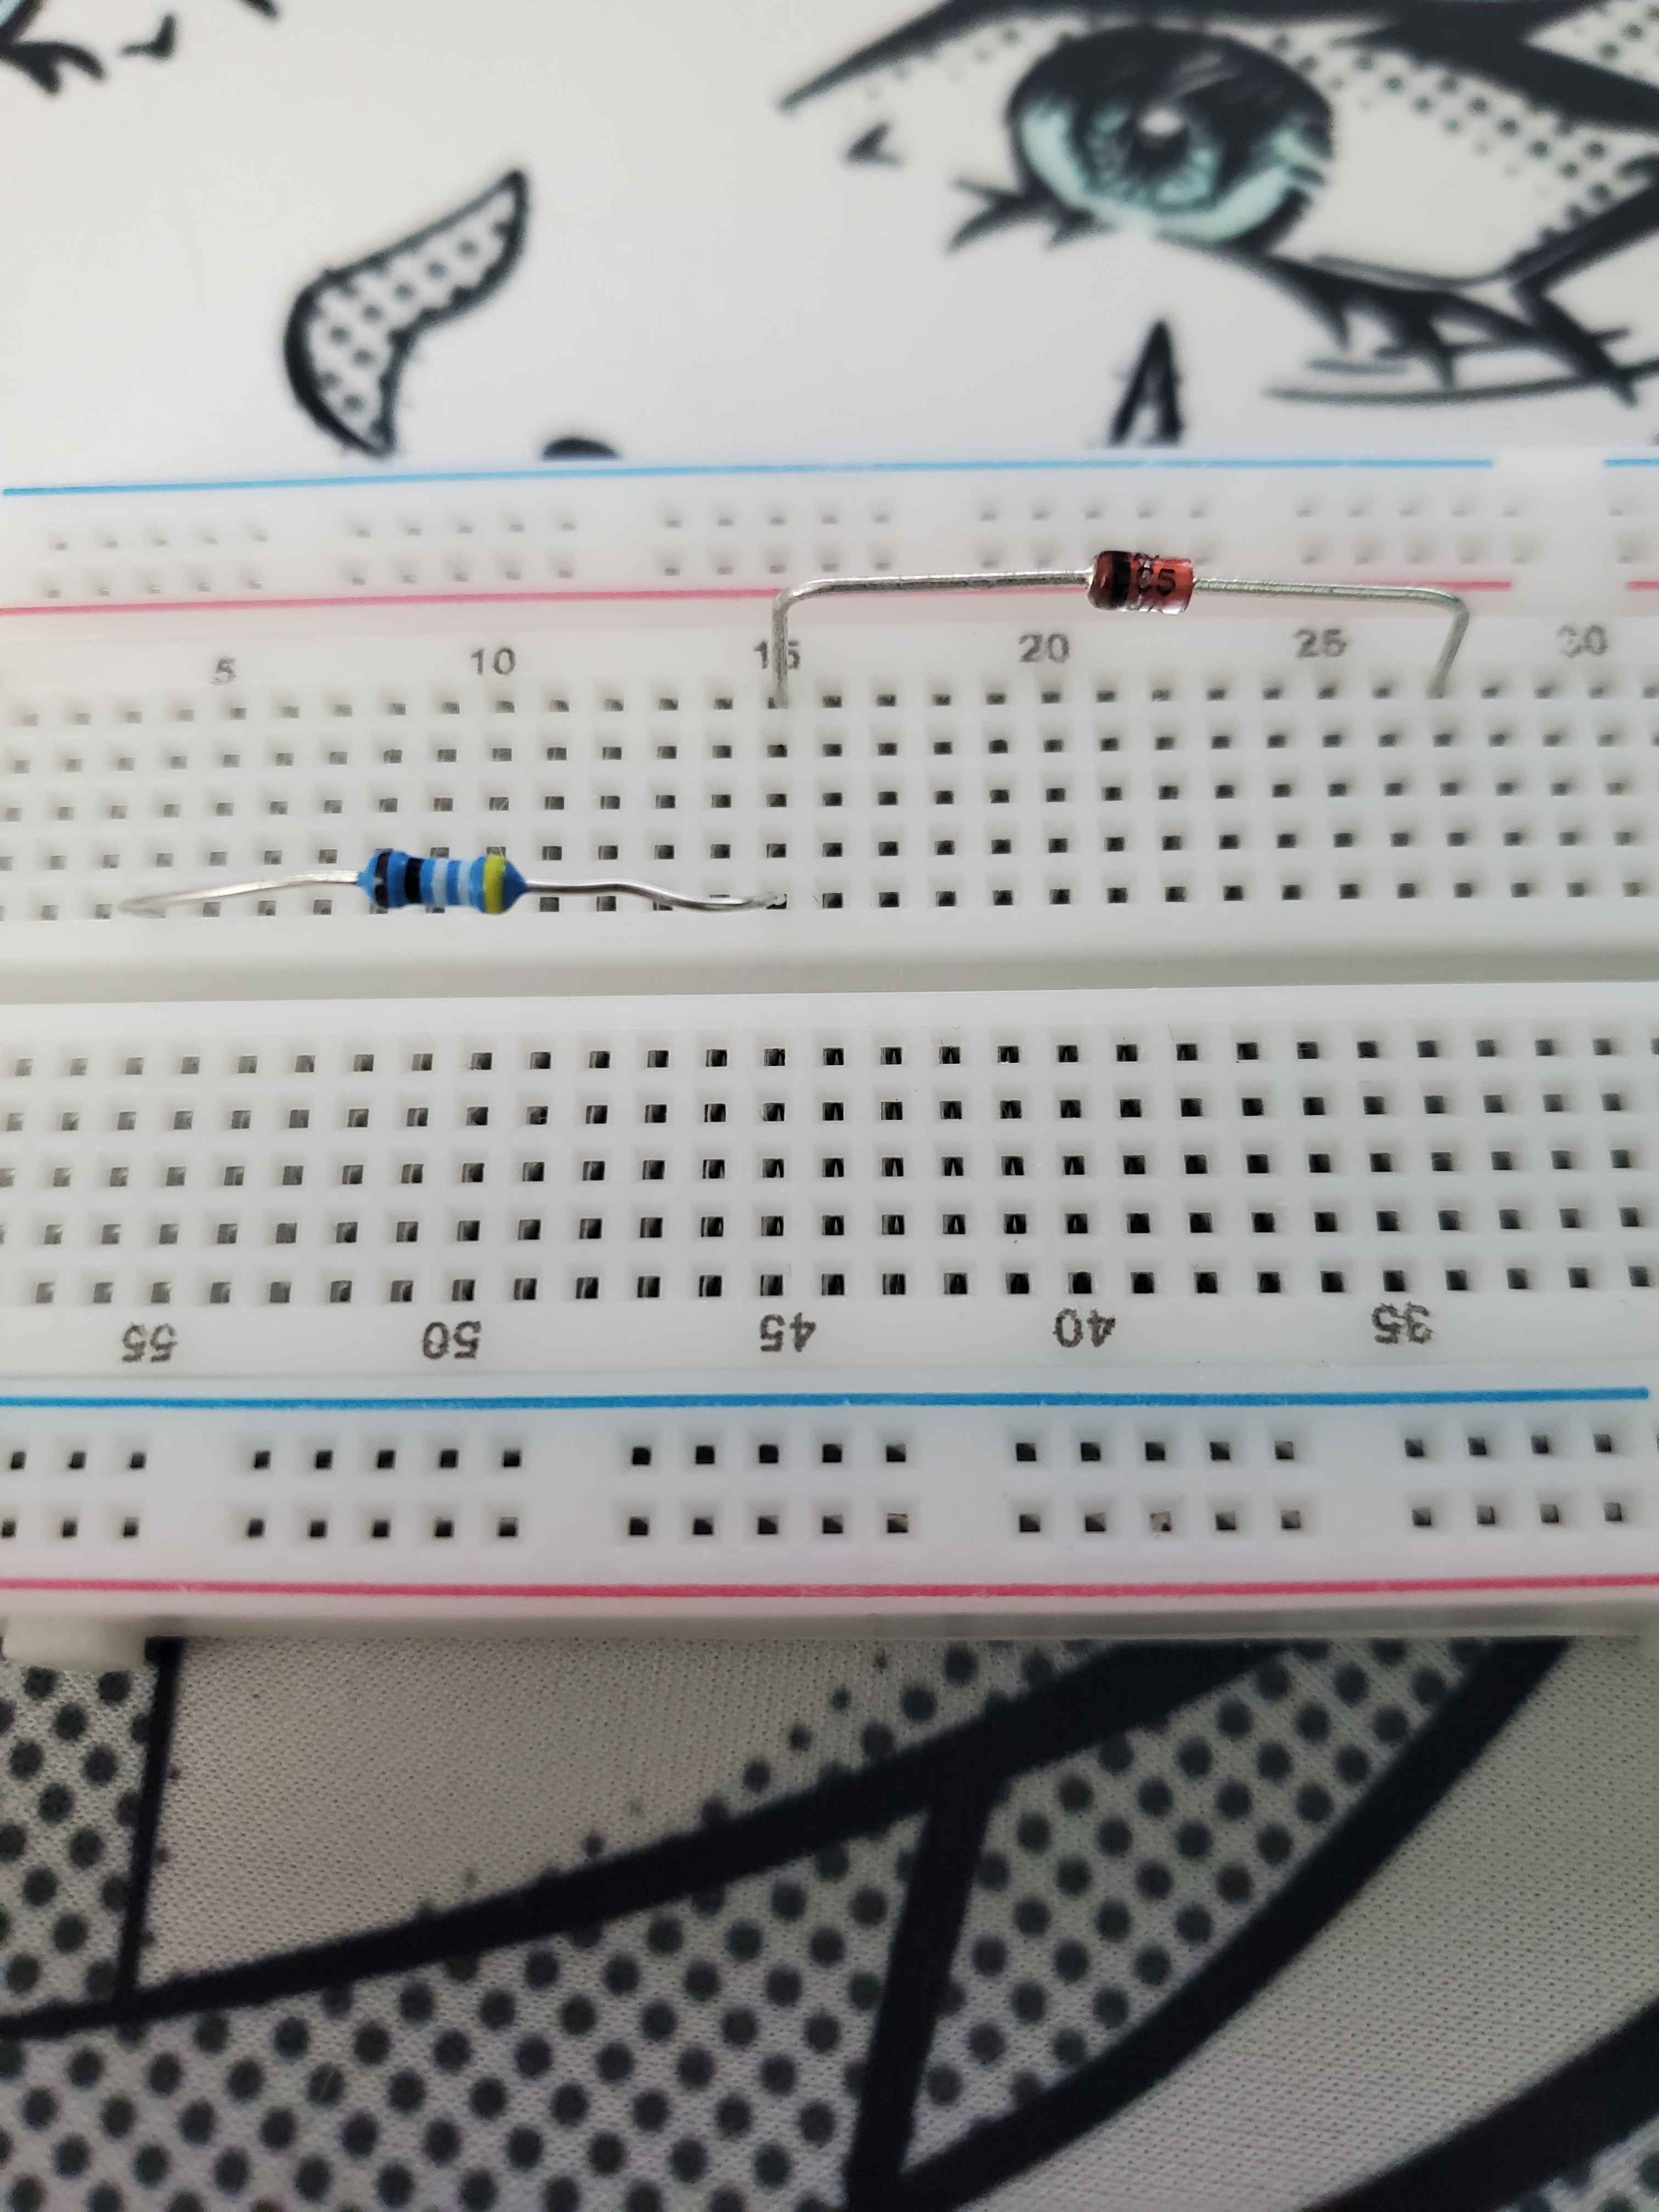
\includegraphics[width=9cm]{20240714_094624}}\hfil
		\subfloat[\centering Series RD Circuit $10k\Omega$]{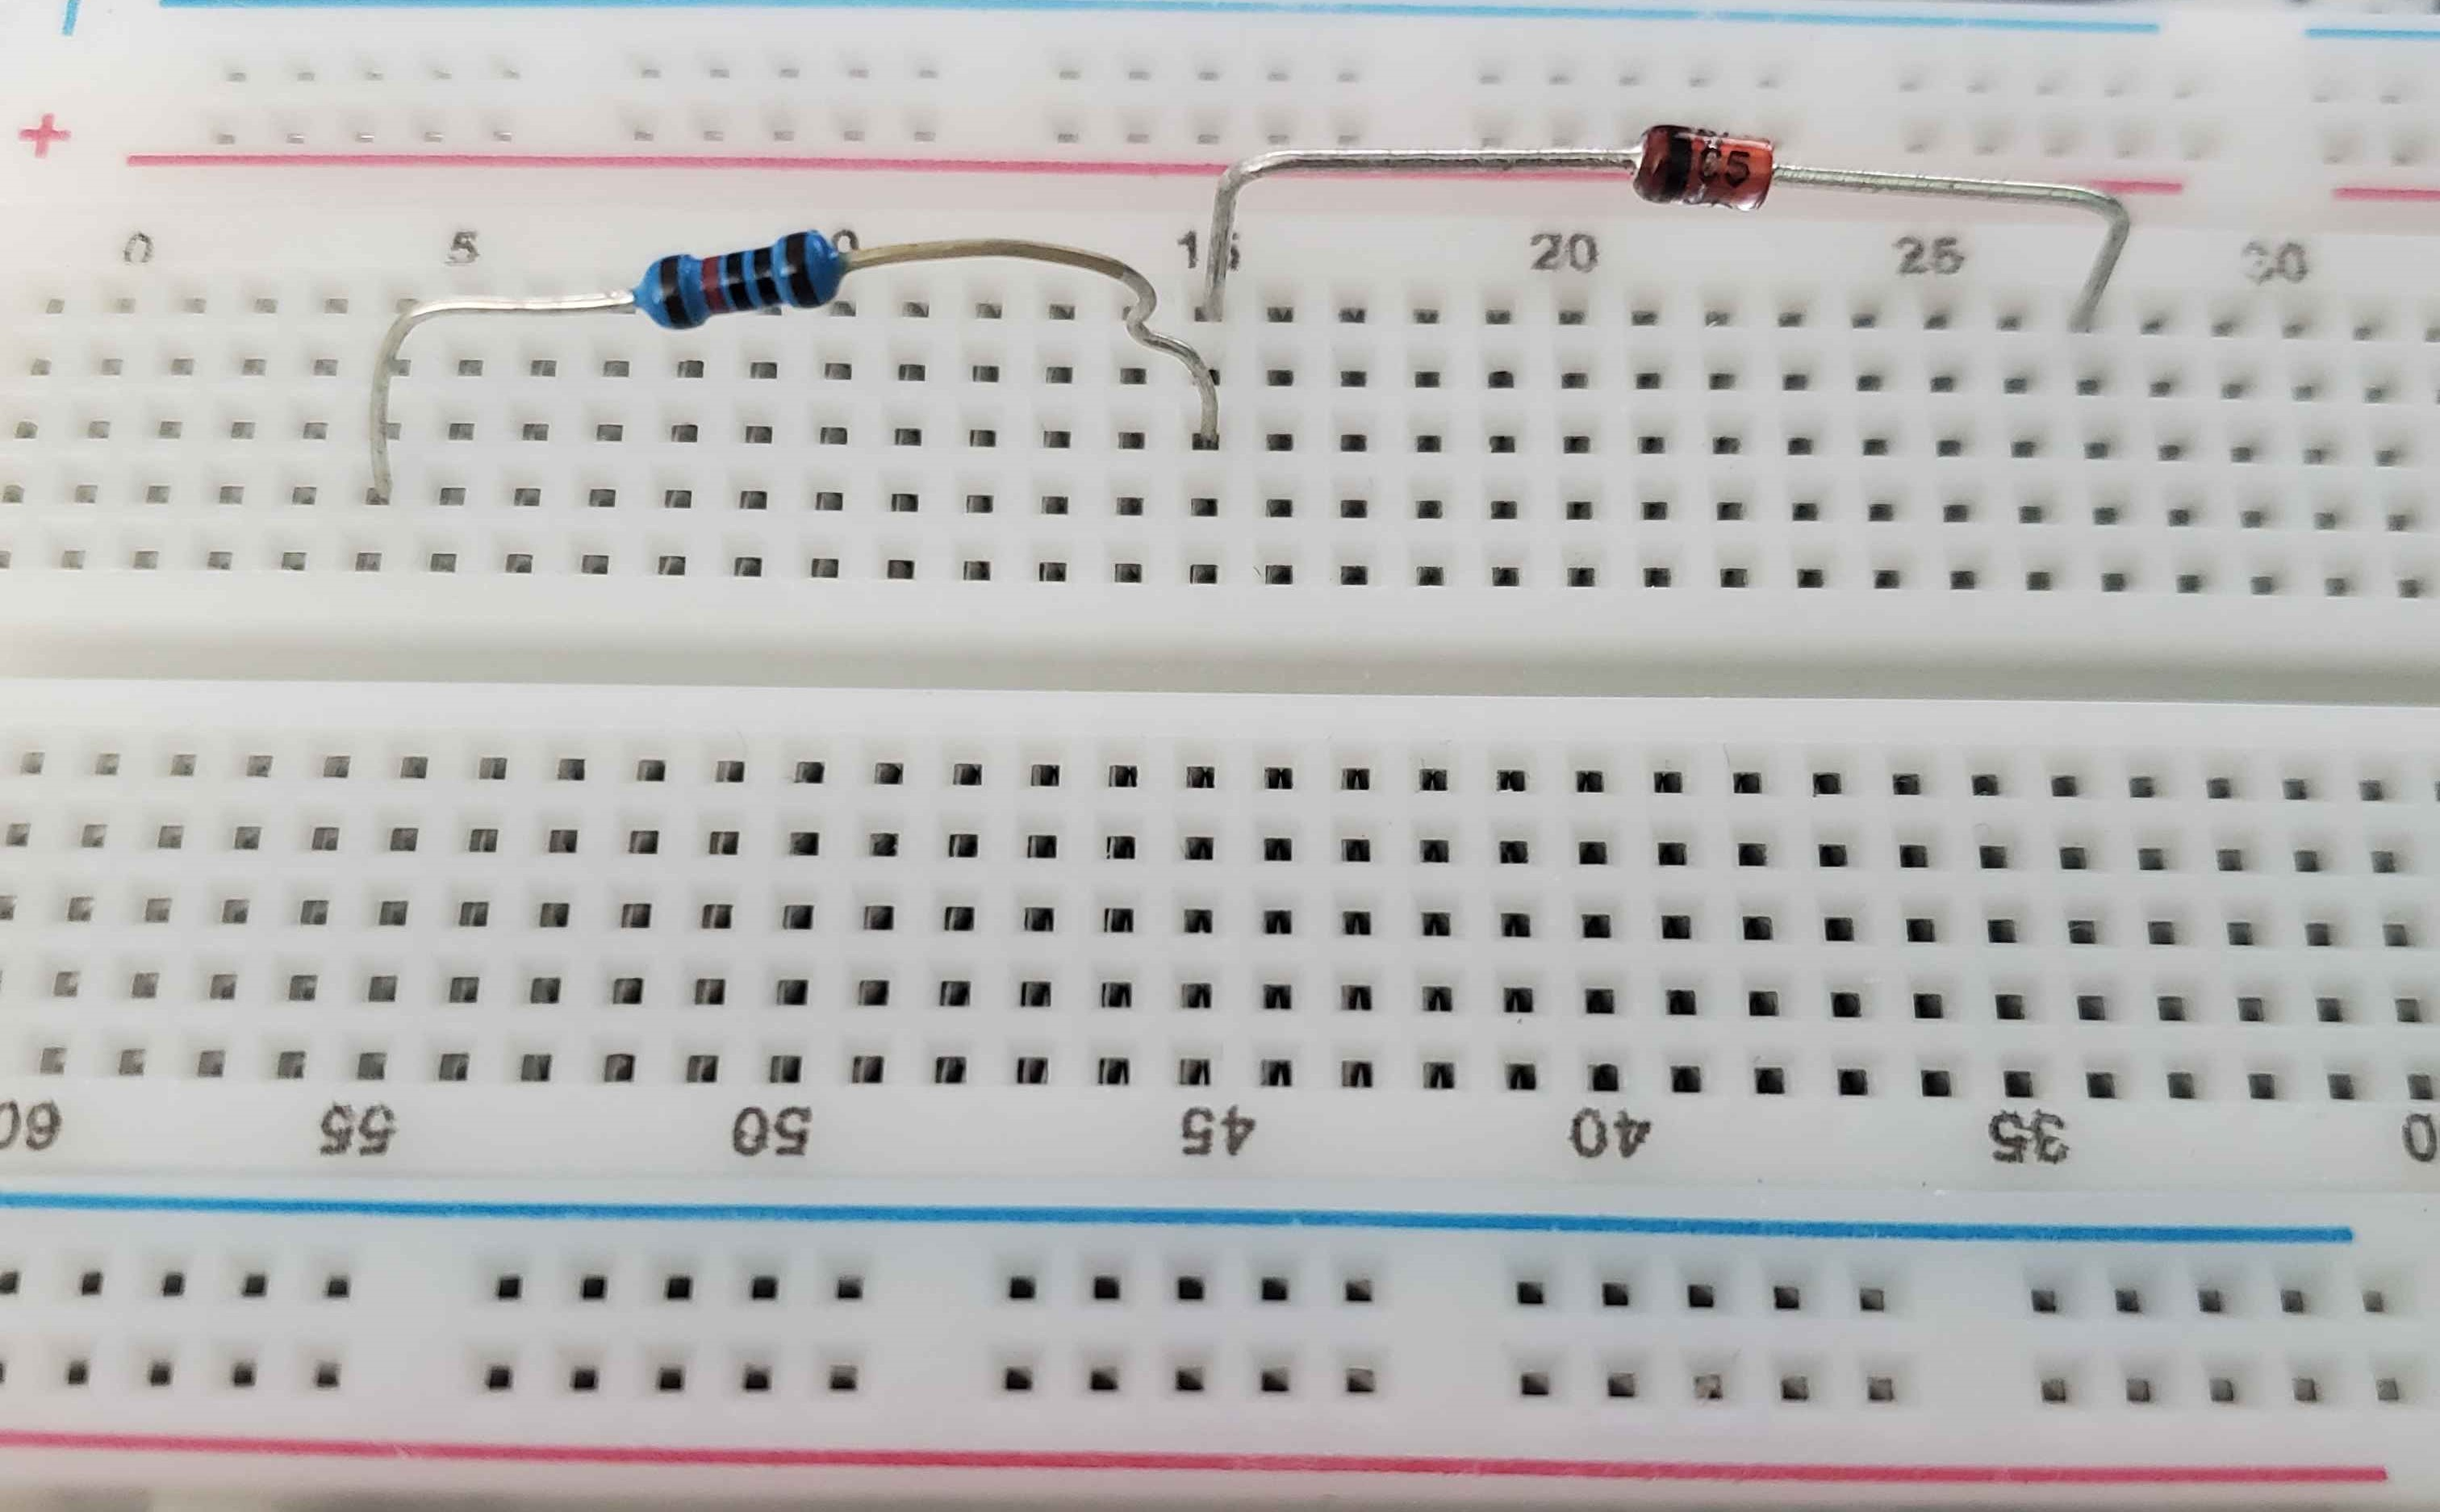
\includegraphics[width=9cm]{20240714_094351}}
	\end{figure}
	\newpage
	\nsection{Descriptions of Measurements \& Calculations}
	Given the default theoretical calculation for a Diode in forward-bias: $I_D=I_S(e^{\frac{V_D}{V_T}}-1)$; the dataset is similar in-nature - not exact because the characteristics of this diode differs - from section 1.1 of the lab.\\
	The characteristic of a \textit{Zener} Diode is its relationship to $-V_D$, as $I_D$ enters \textbf{Reverse-Breakdown} @ $-V_{Z0}$; the point of breakdown.
	\begin{figure}[hp!] %140, 
		\centering
		\caption{$RD_Z$ Circuit}
		\subfloat[RD Circuit Measurement]{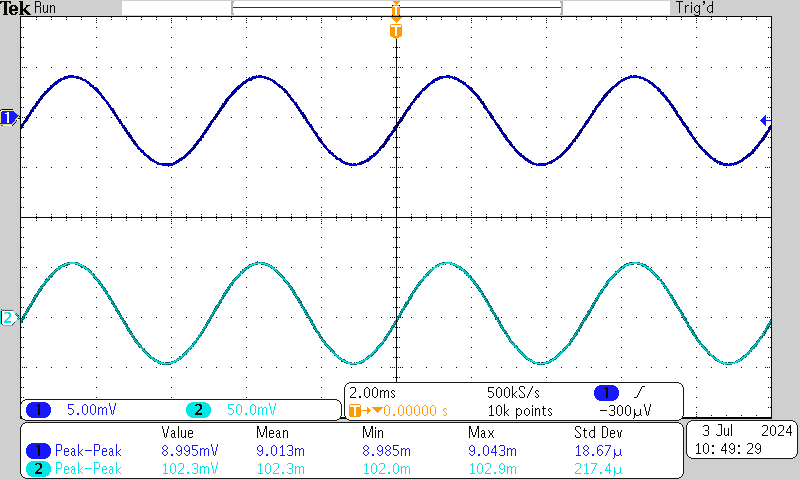
\includegraphics[width=9cm]{tek0000}}
		\subfloat[Sample Measurement ]{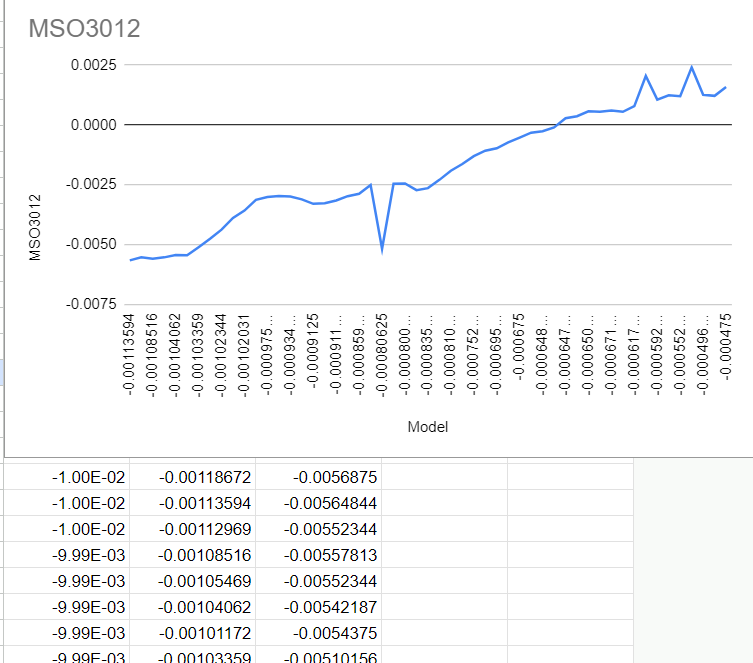
\includegraphics[width=9cm]{Screenshot 2024-07-15 203328}}
	\end{figure}
	\nsection{Summary \& Conclusions}
	Revealed in Figure RD-Circuit 1A \& 1B, the generated oscilloscope readings of the two periodic function match the characteristics of the transfer function found in 1b ($RD_Z$ Circuit). So the measurements do infact closely align.
	\nsubsection{Discussion}
	\begin{itemize}
		\item \textbf{i. Describe how you measured $I_D$ and $V_D$?}
		\subitem At the node where R; ($R>100\Omega$) and the Zener Diode; ($D_Z$) meet, we denote this junction as $V_{out}$. We attach our Multimetre's positive lead (Red) to $V_{out}$, and attached our ground lead to the opposing node of the Zener Diode; ($D_Z$) - which should be grounded.
		\item \textbf{ii. In this experiment how would you determine the value of $I_{D,max}$}
		\subitem \emph{Forward-Bias:} $I_D=I_S(e^{\frac{V_D}{V_T}}-1)$; reference Figure 1b.
		\subitem \emph{Reverse-Breakdown:} The functioning range when $V_D < V_{D_{BR}}$; the output voltage of a reverse-breakdown Zener diode is $V_o=V_i-R_i*_i$ (the subscript of i meaning input of the function generator.)
		\item \textbf{iii. In the circuit, what limits $I_D$?}
		\subitem \emph{Forward-Bias:} The characteristics of the I-V curve of a diode has current $I_D$ exponentially rise towards a cut-off at the threshold, towards the C.V.D @ $V_D$.
		\subitem \emph{Reverse-Breakdown:} Similarly to how the Forward-Bias meets an exponential curve towards its threshold; $V_D$, the Reverse-Breakdown meets and meets a sharp declination of $V_o$ towards $-V_{D_{BR}}$.
		\item \textbf{iv. Explain why $V_D$ does not change much while $I_D$ can change a lot.}
		\subitem Given the equation of a Diode's characteristics of $I_D=I_S(e^{\frac{V_D}{V_T}}-1)$. Putting the equation in reference to $I_D$ is an exponential function, while $V_D$ is a logarithmic function with a very slow rise time. This goes for both Forward-Bias and Reverse-Breakdown, only the output voltage nature changes.
	\end{itemize}
	
		\nchapter{Voltage Limiter Circuits; Standard \& Zener Diode}
	\nsection{Design Objective}
	In this lab, we introduce ourselves to two voltage-limiting circuits. One built with standard diodes and the other built with Zener diodes., we characterise its function by the I-V curve.
	\begingroup
	\renewcommand{\cleardoublepage}{}
	\renewcommand{\clearpage}{}
	\nsection{Circuit Design Outline}
	\endgroup
	With a resistor of an arbitrary impedance greater than $100\Omega$ ($R\geq100\Omega$), and the natural impedance of the Function Generator in series ($R_{TOT}=R_{FG}+R\geq150\Omega$), the designed High-Level Limiter Circuit is set in series to the resistor; through the function generator. Set the function generator @ f=200kHz and $V_P=5V,0.1V,10V$ in High-Z impedance.
	\begin{figure}[h!]
		\centering
		\caption{\centering High-Level Limiter Circuit}
		\subfloat[\centering Rudimentary Generic Schematic of High-level Limiter Circuit]{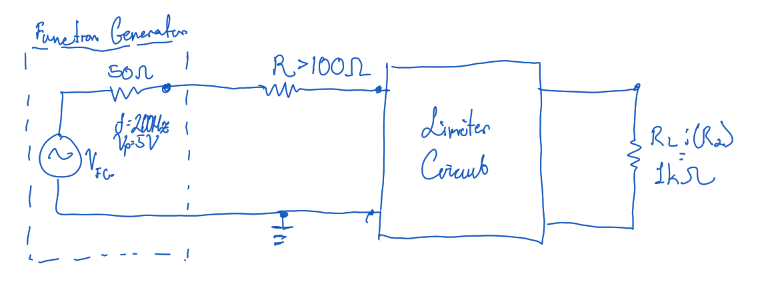
\includegraphics[width=19cm]{Screenshot 2024-07-15 211530}}
	\end{figure}
	\begin{figure}[h!]
		\ContinuedFloat
		\centering
		\subfloat[\centering LTSpice + Rudimentary Schematic Parallel Standard Diodes Circuit]{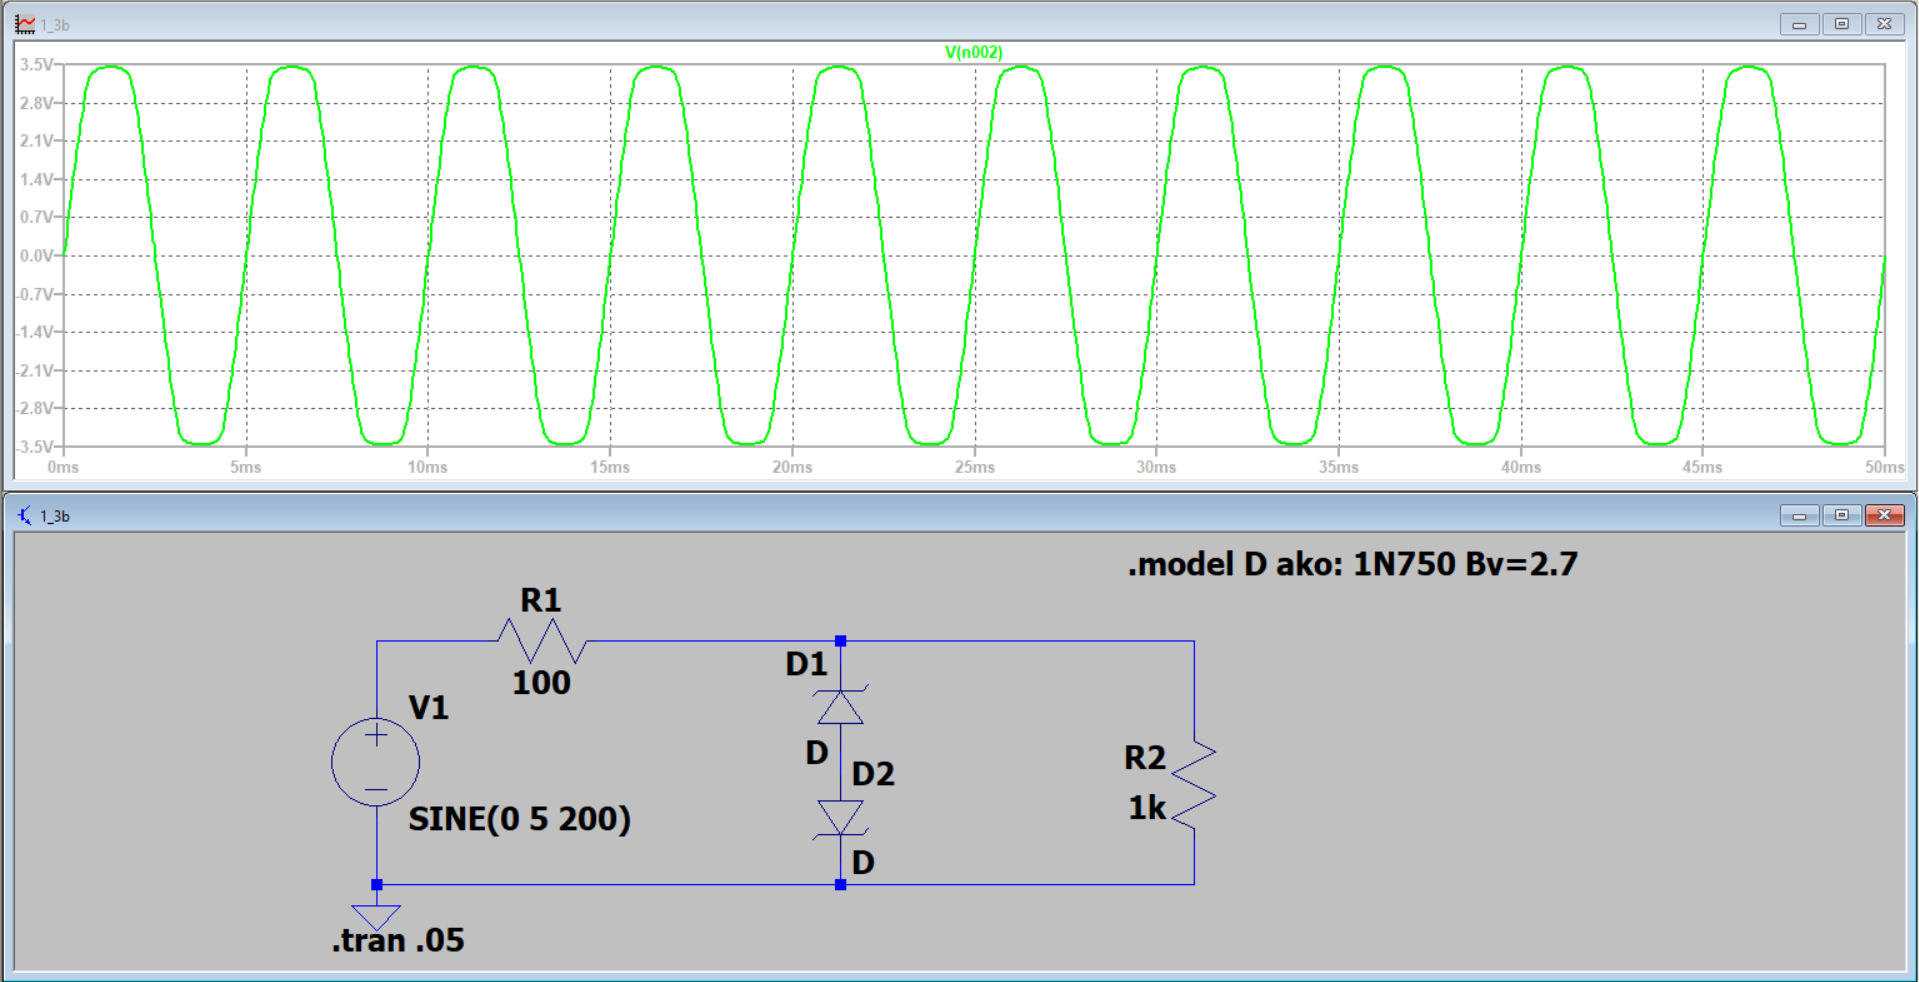
\includegraphics[width=9cm]{Screenshot 2024-07-15 063021}}
		\subfloat[\centering LTSpice + Rudimentary Schematic Series Opposing Zener Diodes Circuit]{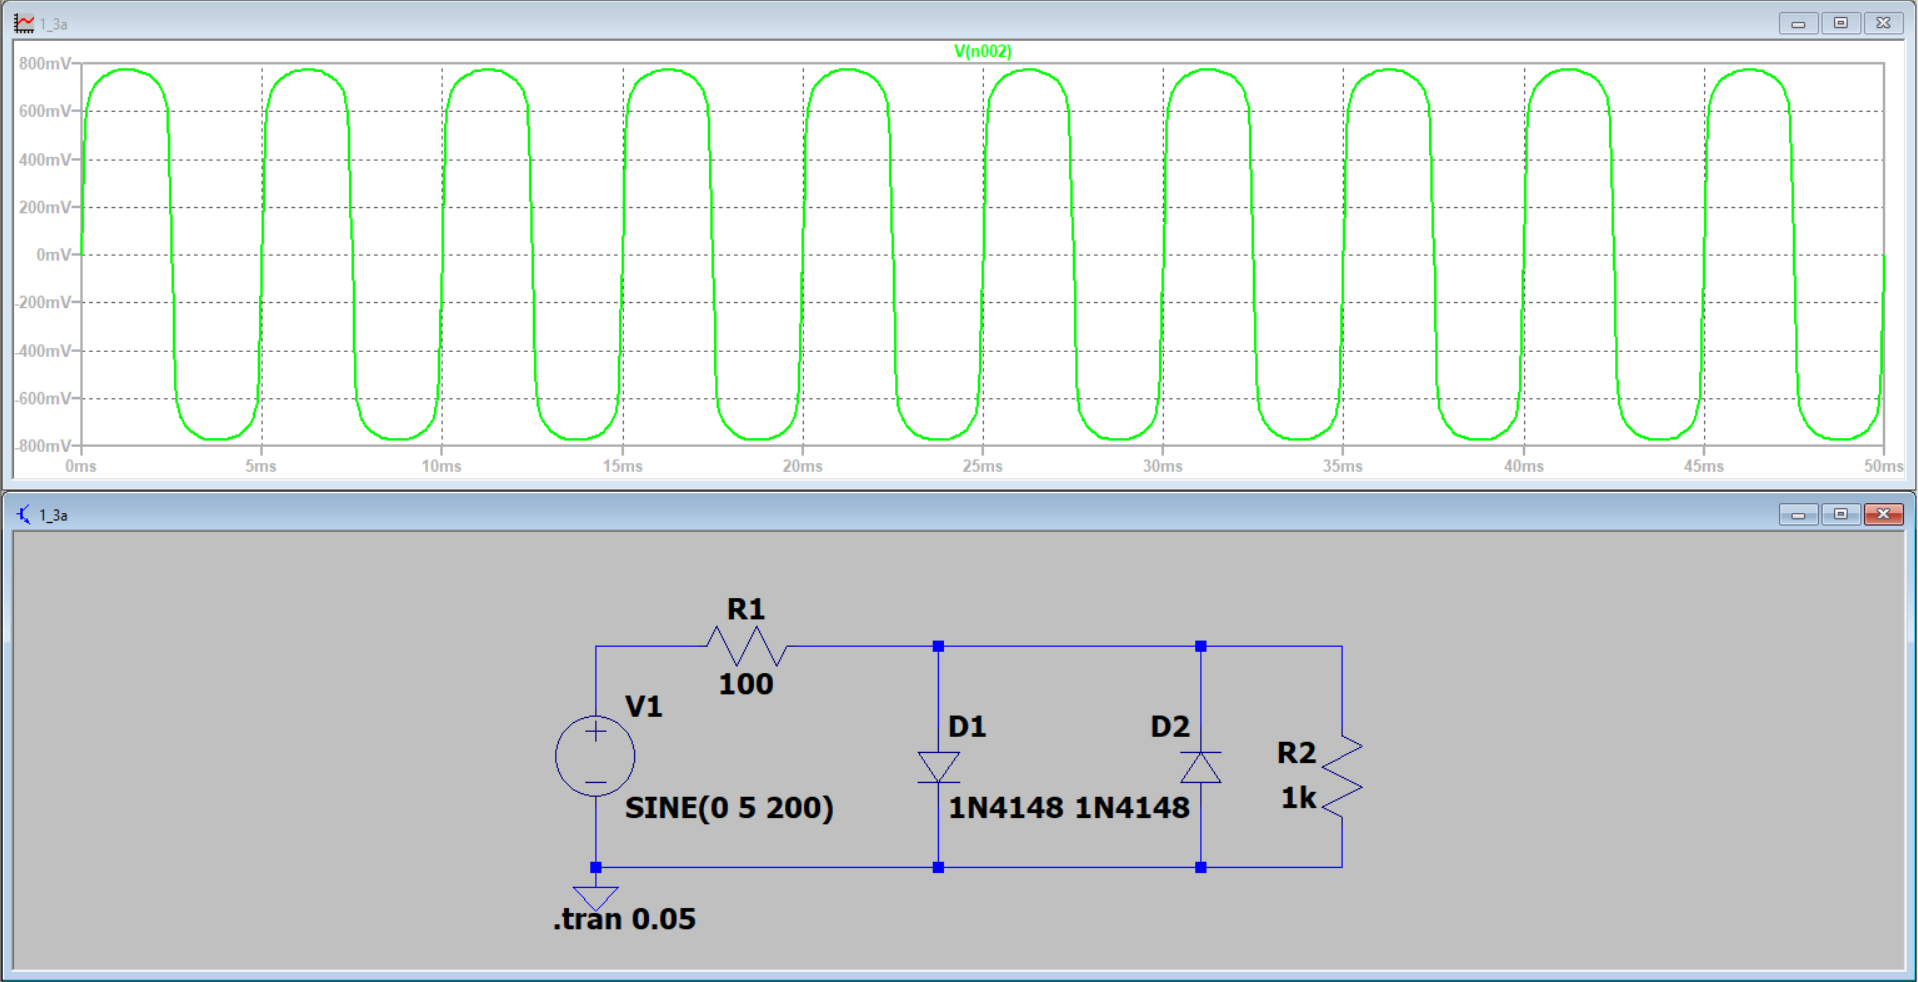
\includegraphics[width=9cm]{Screenshot 2024-07-15 063246}}
	\end{figure}
	\begin{figure}[h!]
		\ContinuedFloat
		\centering
		\subfloat[\centering Parallel Standard Diodes Circuit]{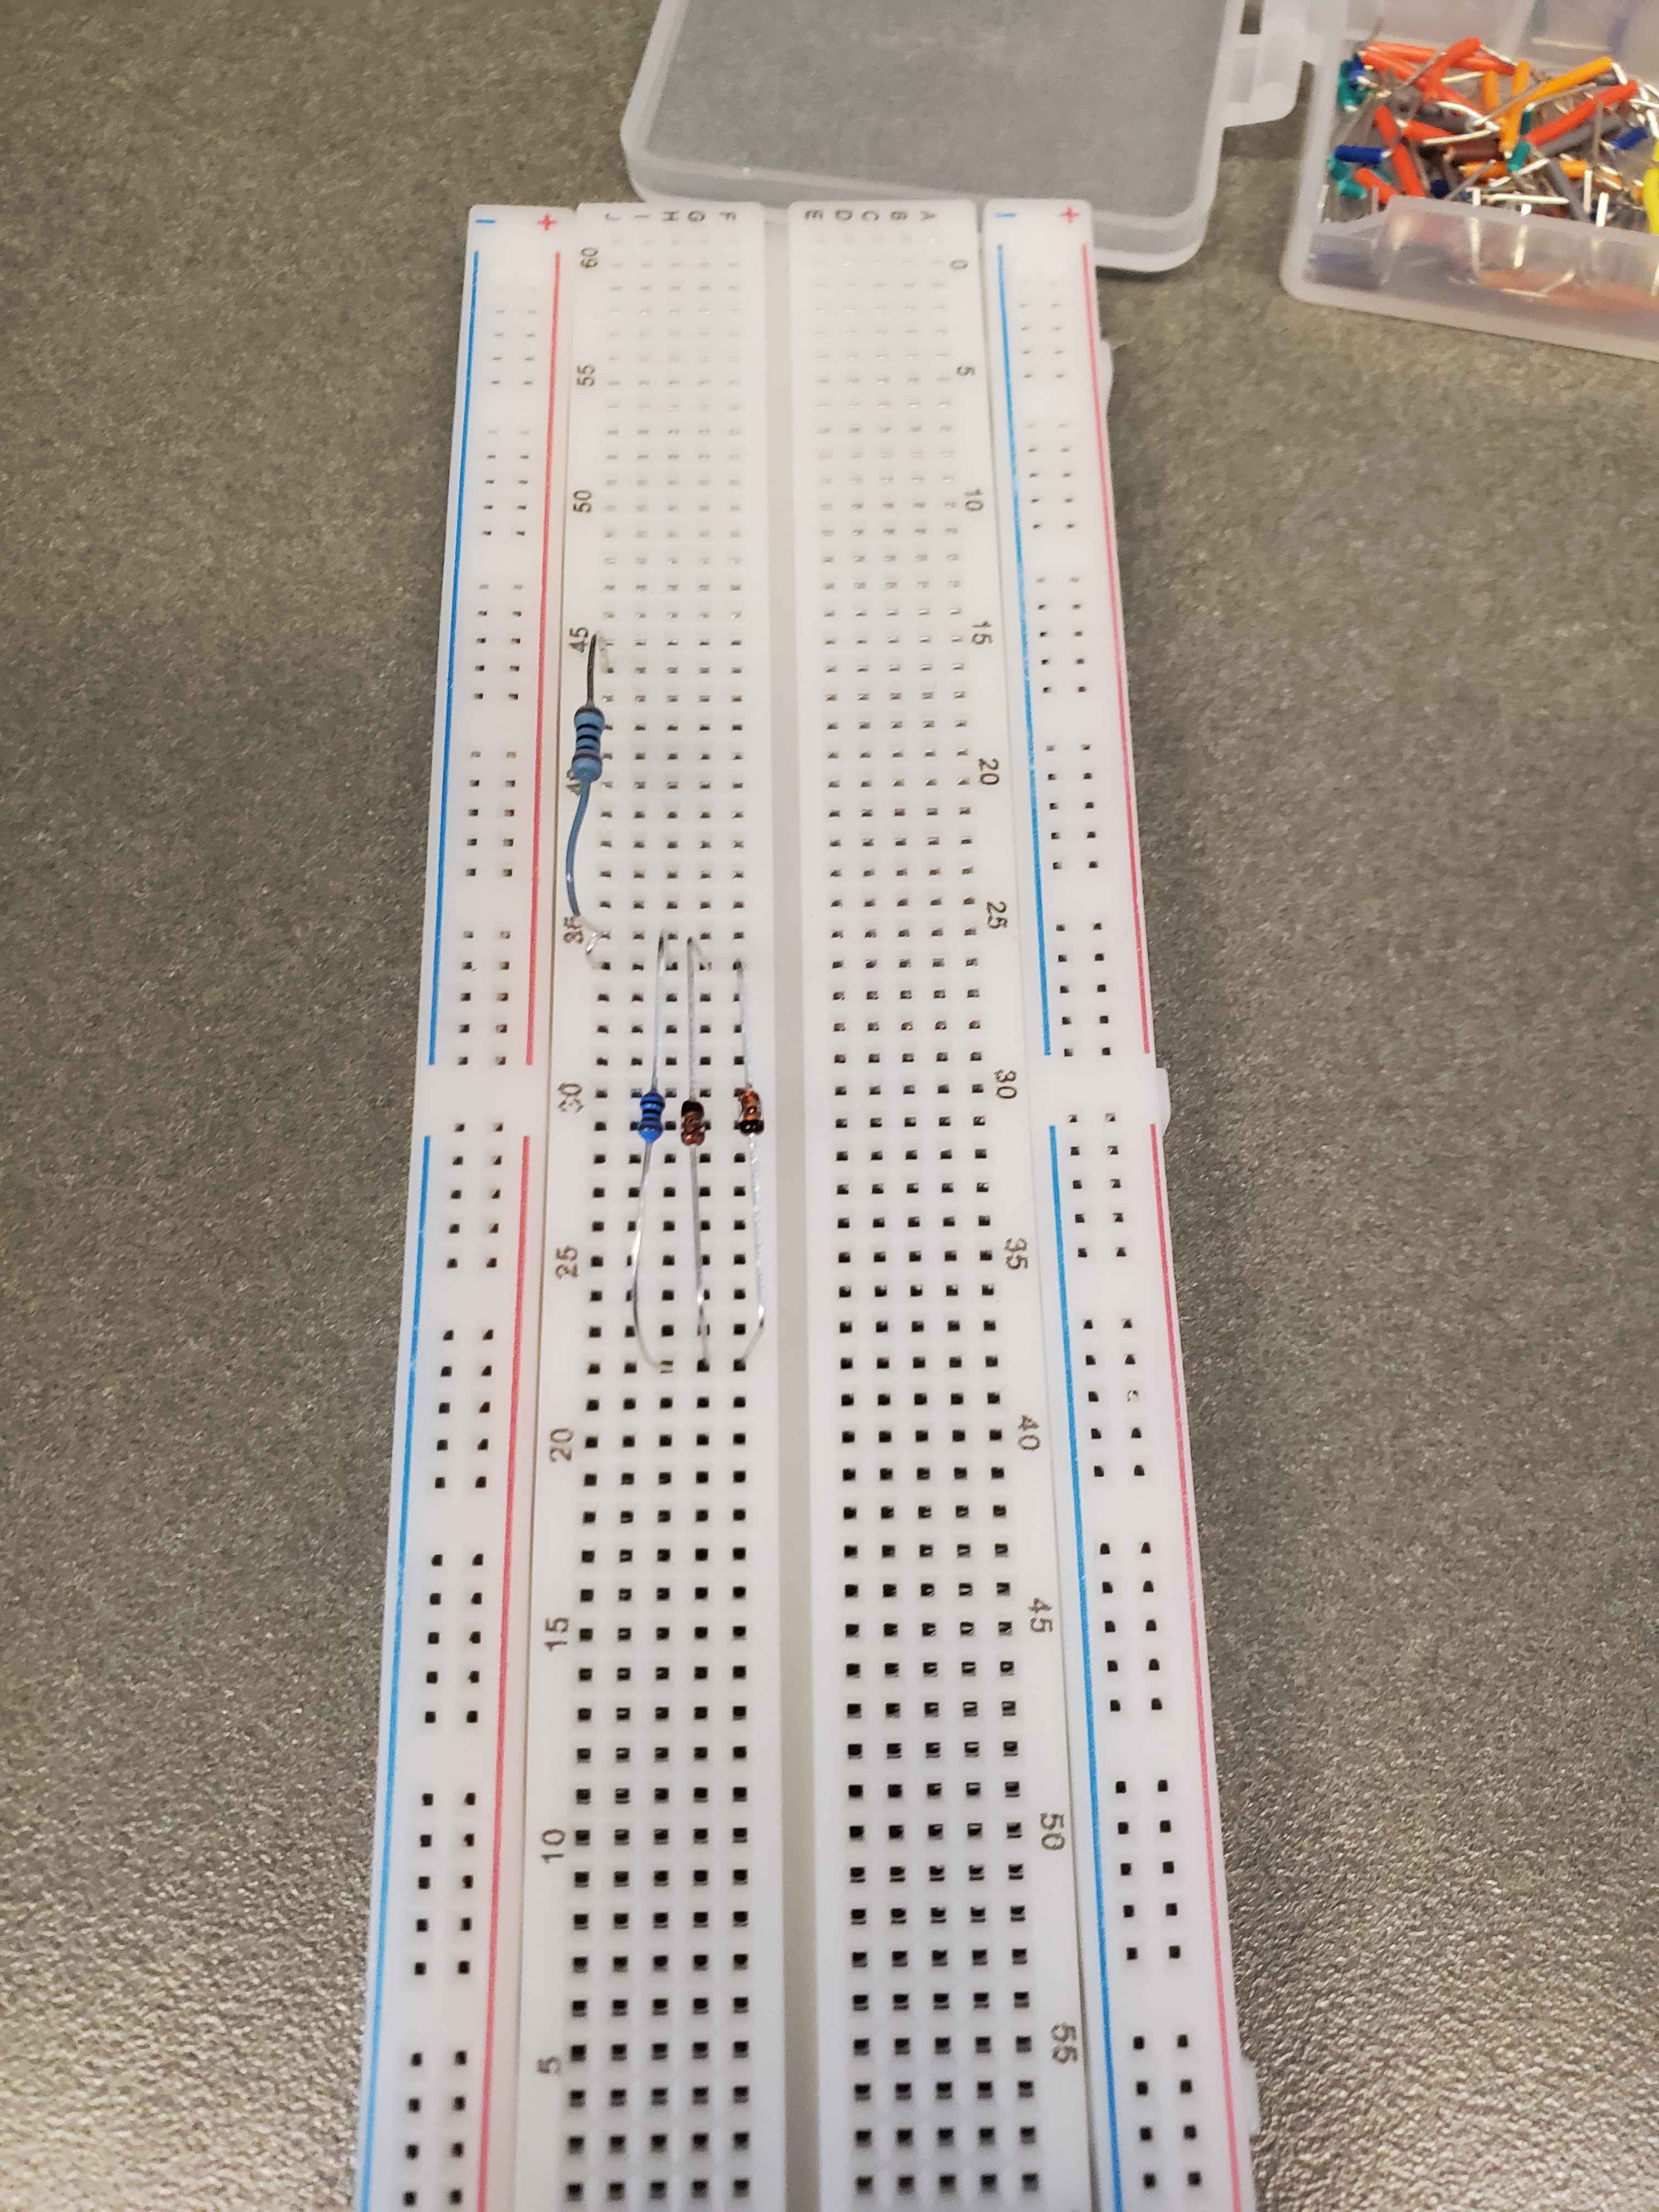
\includegraphics[width=9cm]{20240703_124842}}\hfil
		\subfloat[\centering Series Opposing Zener Diodes Circuit]{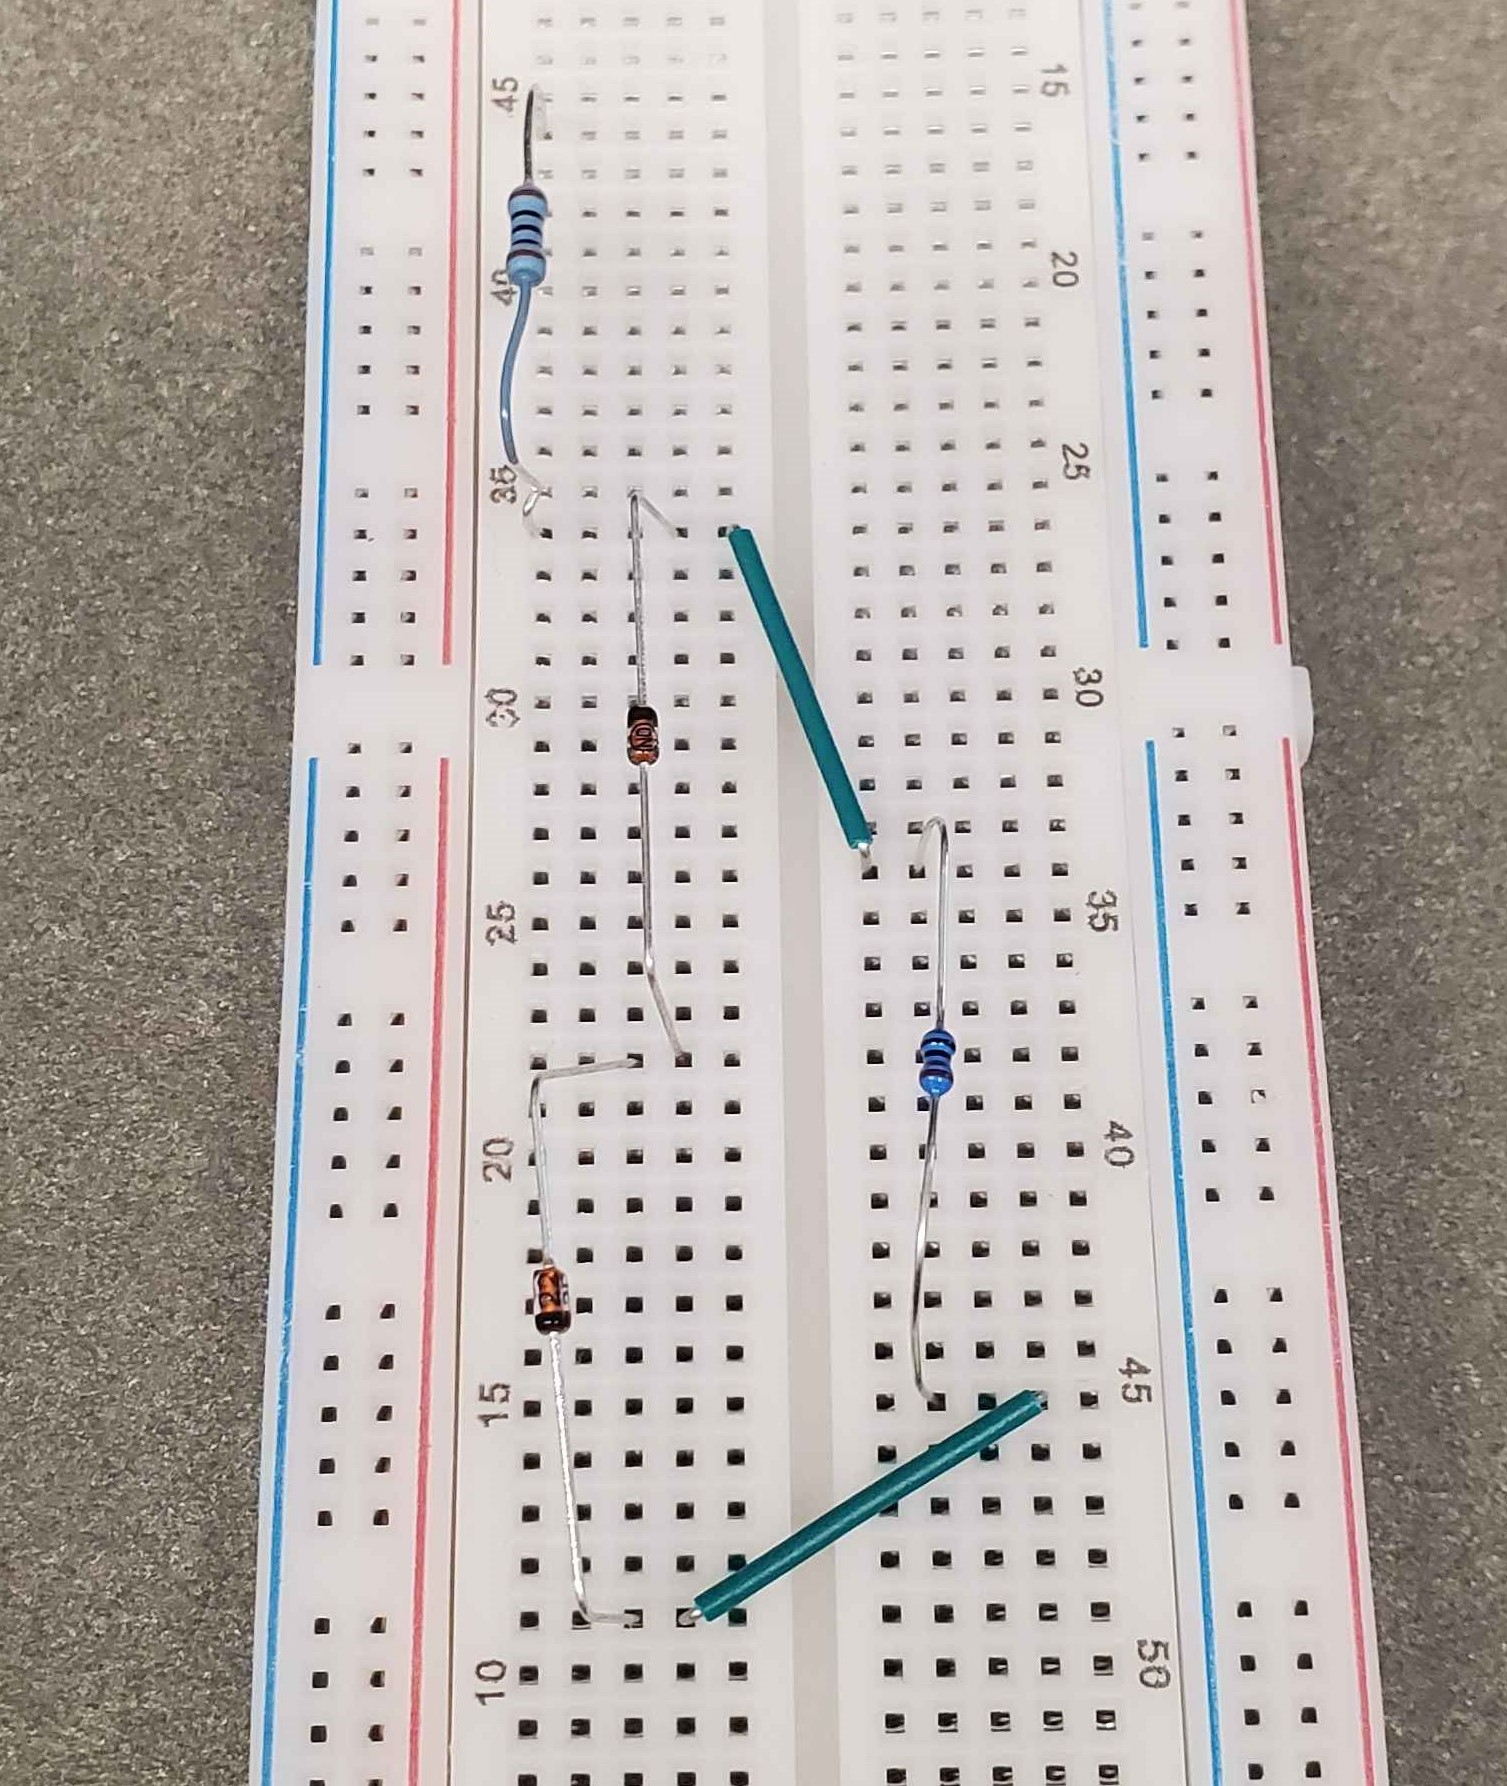
\includegraphics[width=9cm]{20240703_124754}}
	\end{figure}
	
	\newpage
	
	\nsection{Descriptions of Measurements \& Calculations}
	Given the default theoretical calculation for a Diode in forward-bias: $I_D=I_S(e^{\frac{V_D}{V_T}}-1)$; the dataset is similar in-nature - not exact because the characteristics of this diode differs - from section 1.1 of the lab.\\
	The characteristic of a \textit{Zener} Diode is its relationship to $-V_D$, as $I_D$ enters \textbf{Reverse-Breakdown} @ $-V_{Z0}$; the point of breakdown.\\
	Because of these characteristics, the Limiter-Circuits meet their respective "off" thresholds to logarithmically degrade the output voltage of $V_o$.
	\begin{figure}[h!] %140, 
		\centering
		\caption{High-Limiter Circuit Scope}
		\subfloat[Parallel RDD Circuit @ $0.1V_p$]{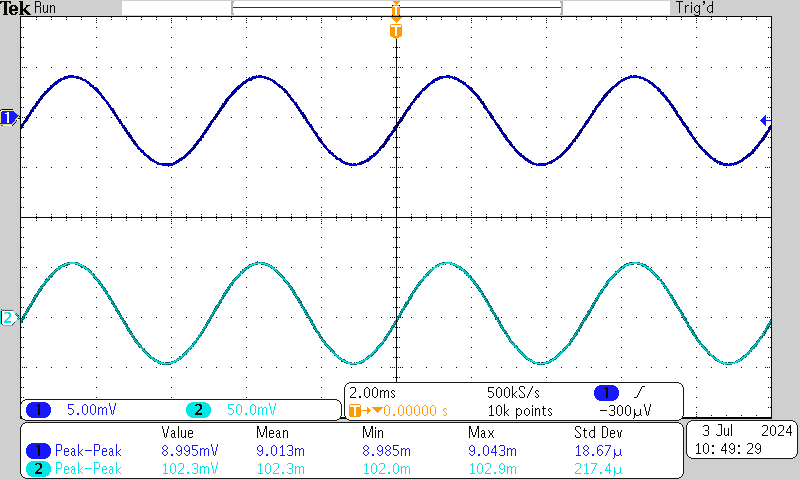
\includegraphics[width=8cm]{tek0000}}\hfil
		\subfloat[Parallel RDD Circuit @ $10V_p$]{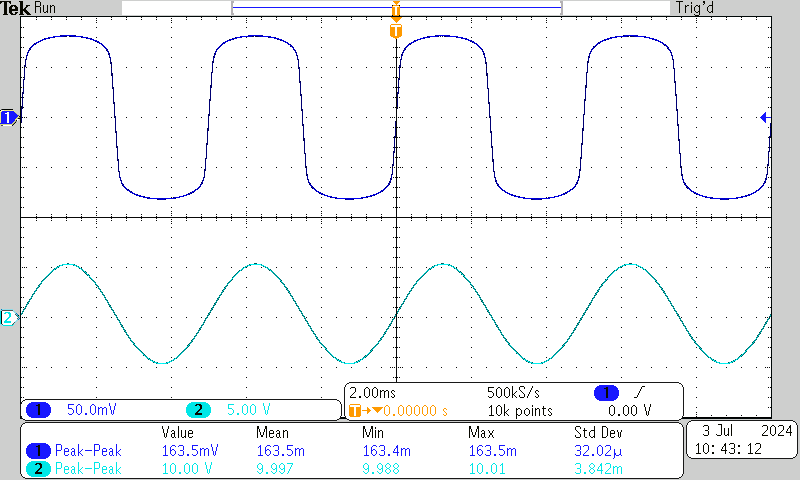
\includegraphics[width=8cm]{tek0001}}\hfil
		\subfloat[Series Opposing-Polarity Zener Diode Circuit @ $0.1V_p$]{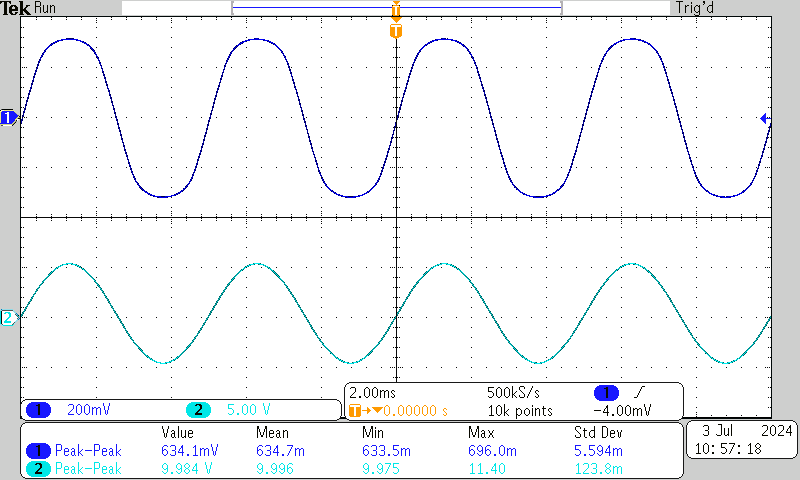
\includegraphics[width=8cm]{tek000000}}\hfil
		\subfloat[Series Opposing-Polarity Zener Diode Circuit @ $10V_p$]{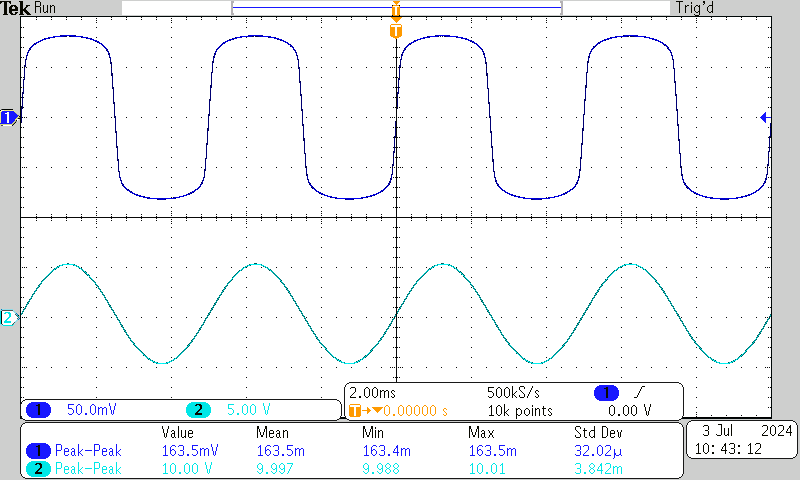
\includegraphics[width=8cm]{tek0001}}
	\end{figure}
	\nsection{Summary \& Conclusions}
	Revealed in Figure RDD-Circuit 0A \& 0B, the generated oscilloscope readings of the two periodic function do in-fact dampen @ $V_{in}$ (CH2) greatly to $V_{out}$ (CH1). It is similary in the Series $D_Z$ circuit.
	\nsubsection{Discussion}
	\begin{itemize}
		\item \textbf{i. Describe how each limiter circuit limits the input voltage based on the output waveform you measured. How are the limiter circuits 1 and 2 different?}
		\subitem The first limiter circuit reduces peak voltage showing the behavior of the exponential diodes. This makes the output wave more square than the input wave because it is limiting the input before it can start curving back down. [Reference Above]
		\item \textbf{ii. What is the effect of setting the \textit{Load Impedance to High Z} mode for the function generator?}
		\subitem \emph{Forward-Bias:} $I_D=I_S(e^{\frac{V_D}{V_T}}-1)$; reference Figure 1b.
		\subitem The instrument will display less attenuation when producing the signal; so in ley, less of a impeded signal.
		\item \textbf{iii. What settings did you use in the oscilloscope in order to suppress noises in the output signals??}
		\subitem \emph{Forward-Bias:} The characteristics of the I-V curve of a diode has current $I_D$ exponentially rise towards a cut-off at the threshold, towards the C.V.D @ $V_D$.
		\subitem High-Fine, Auto-range, 50\% auto-trigger, AC-Coupling.
		\item \textbf{iv. For the limiter Circuit 1, can you make the output signal the same as the input signal by changing $v_{peak}$}
		\subitem You should be able to make the output signal the same by staying in the region where both diodes are in an "off" state. This will cause the circuit to not be limited by current through the diodes.
	\end{itemize}
	
		\nchapter{Full-Wave Bridge Rectifier Circuit}
	\nsection{Design Objective}
	In this lab, we introduce ourselves to two voltage rectifying circuits: The Rectifier and Voltage Clamp. We demonstrated this two two applications across 3 circuits. We characterize its function in $V_{out}$.
	\begingroup
	\renewcommand{\cleardoublepage}{}
	\renewcommand{\clearpage}{}
	\nsection{Circuit Design Outline}
	\endgroup
	[Guidelines do not ask for explanation on design. See Below.]
	\begin{figure}[h!]
		\centering
		\caption{Bridge Rectifier Circuits}
		\subfloat[\centering LTSpice + Rudimentary Schematic Full-Wave Bridge Rectifier]{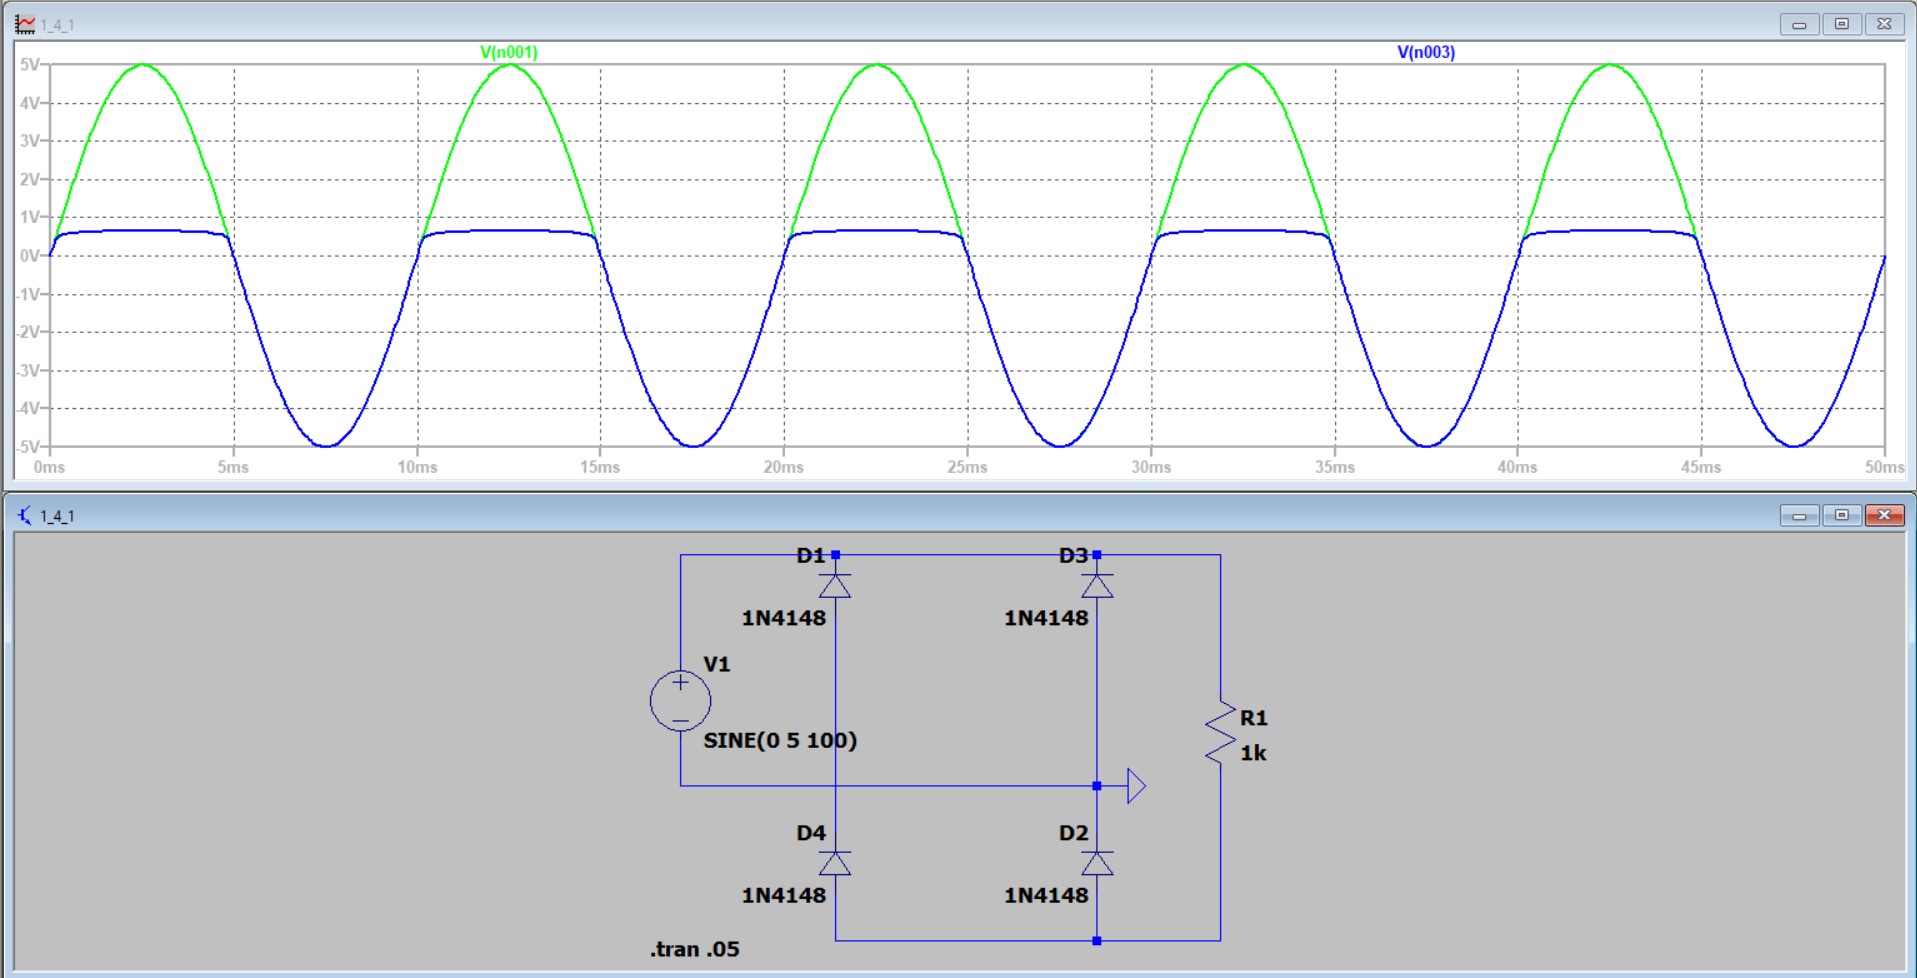
\includegraphics[width=9cm]{Screenshot 2024-07-15 062842}}\hfil
		\subfloat[\centering LTSpice + Rudimentary Schematic Full-Wave Bridge Rectifier with output filter]{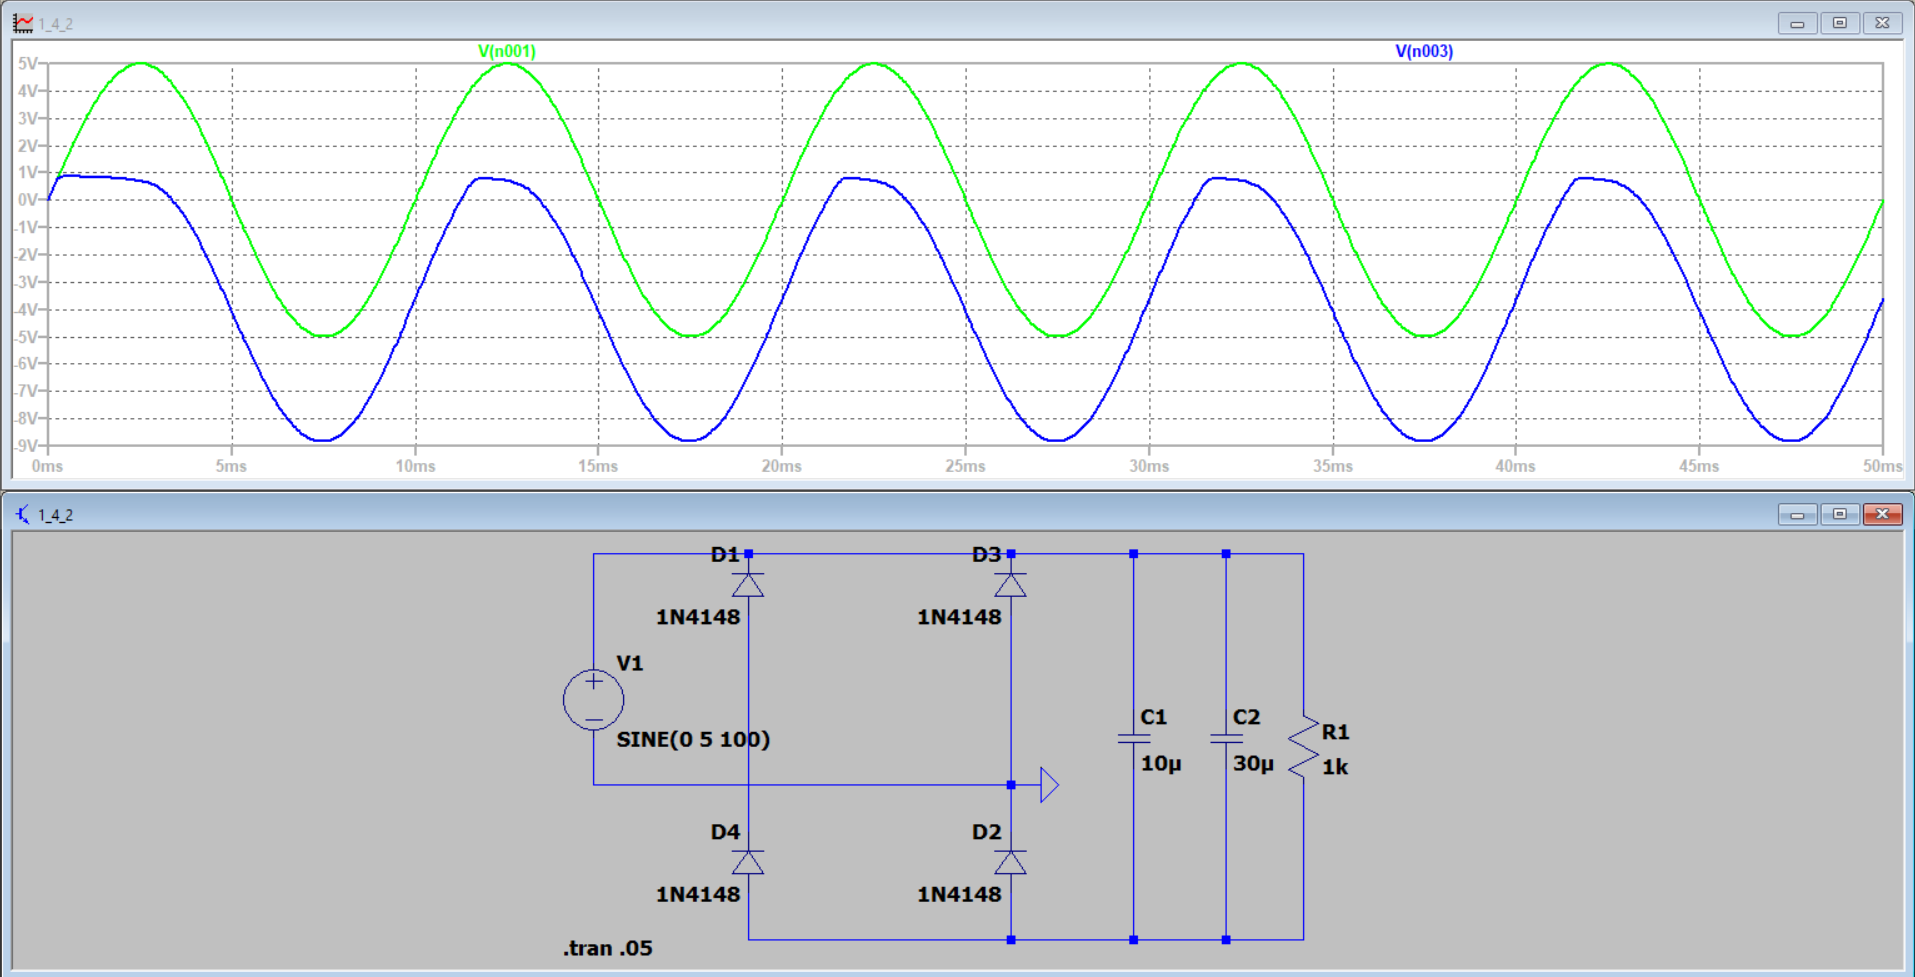
\includegraphics[width=9cm]{Screenshot 2024-07-15 062809}}\hfil
		\subfloat[\centering LTSpice + Rudimentary Schematic Full-Wave Bridge Rectifier with output filter and Zener diode regulator as its output]{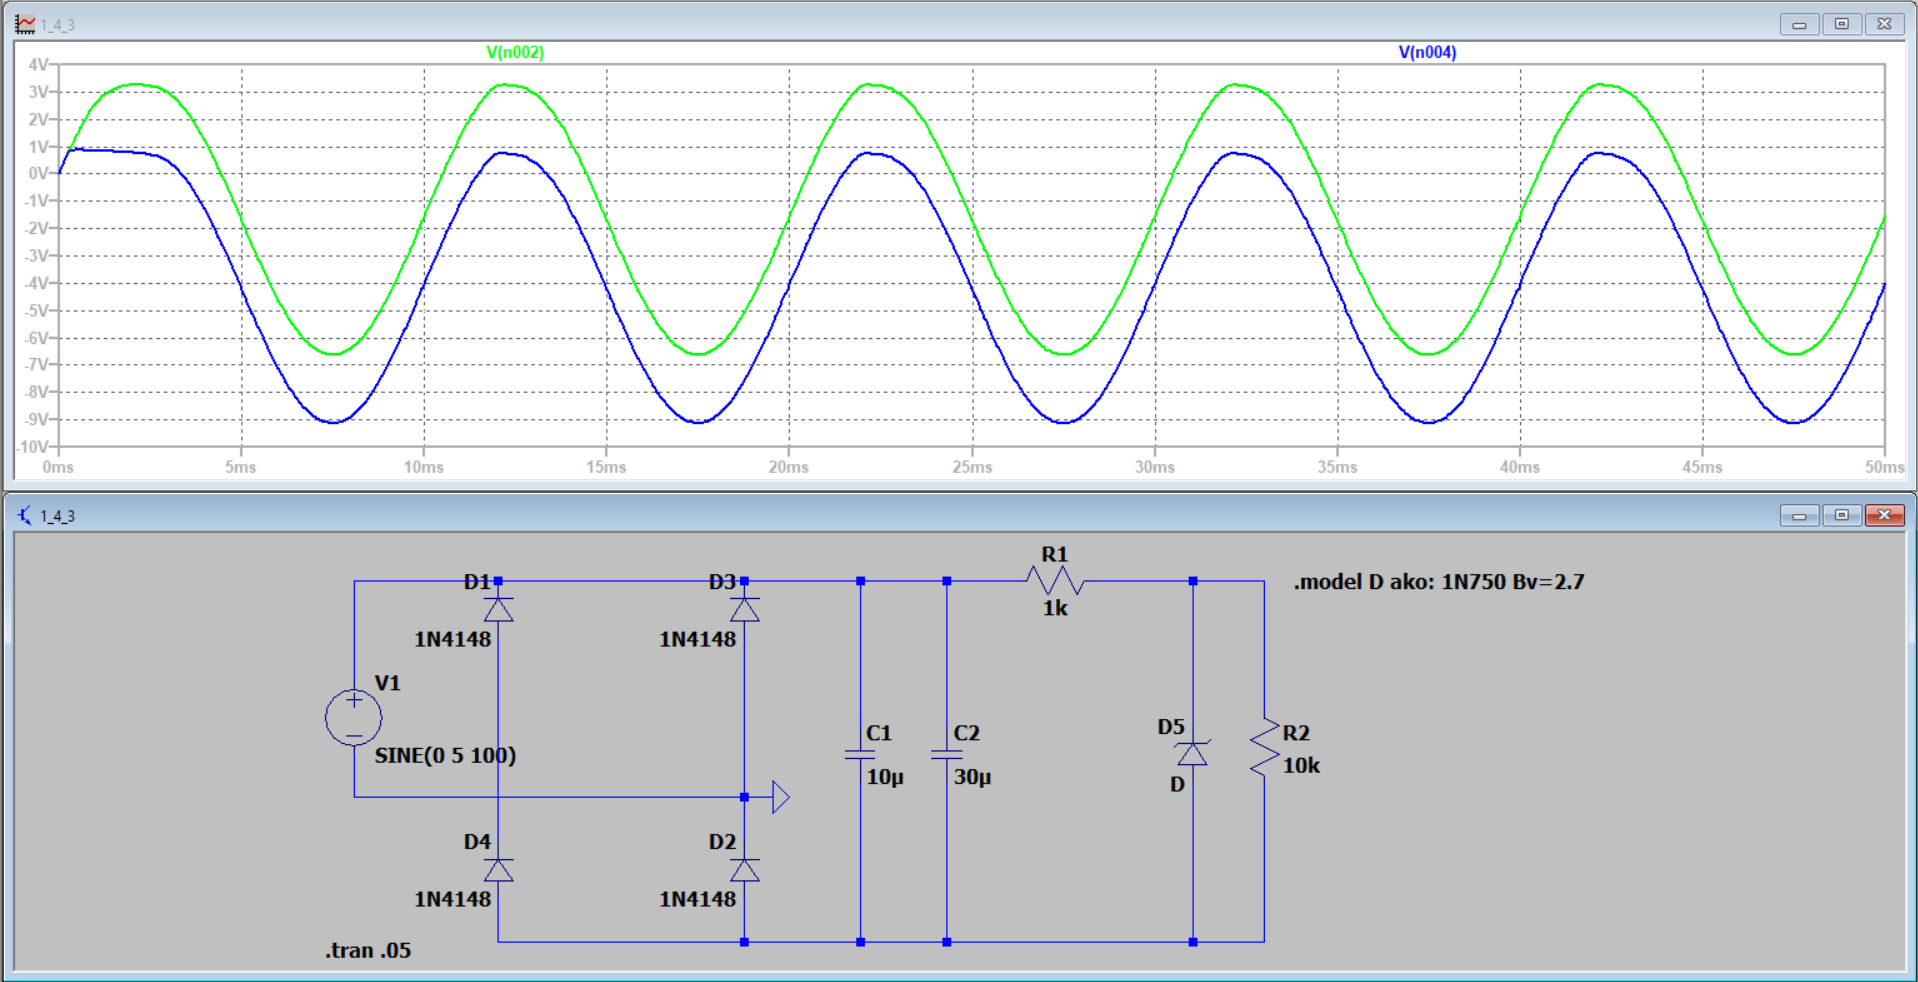
\includegraphics[width=9cm]{Screenshot 2024-07-15 062905}}
	\end{figure}
	
	\begin{figure}[h!]
		\centering
		\caption{Bridge Rectifier Circuits IRL}
		\subfloat[\centering Full-Wave Bridge Rectifier]{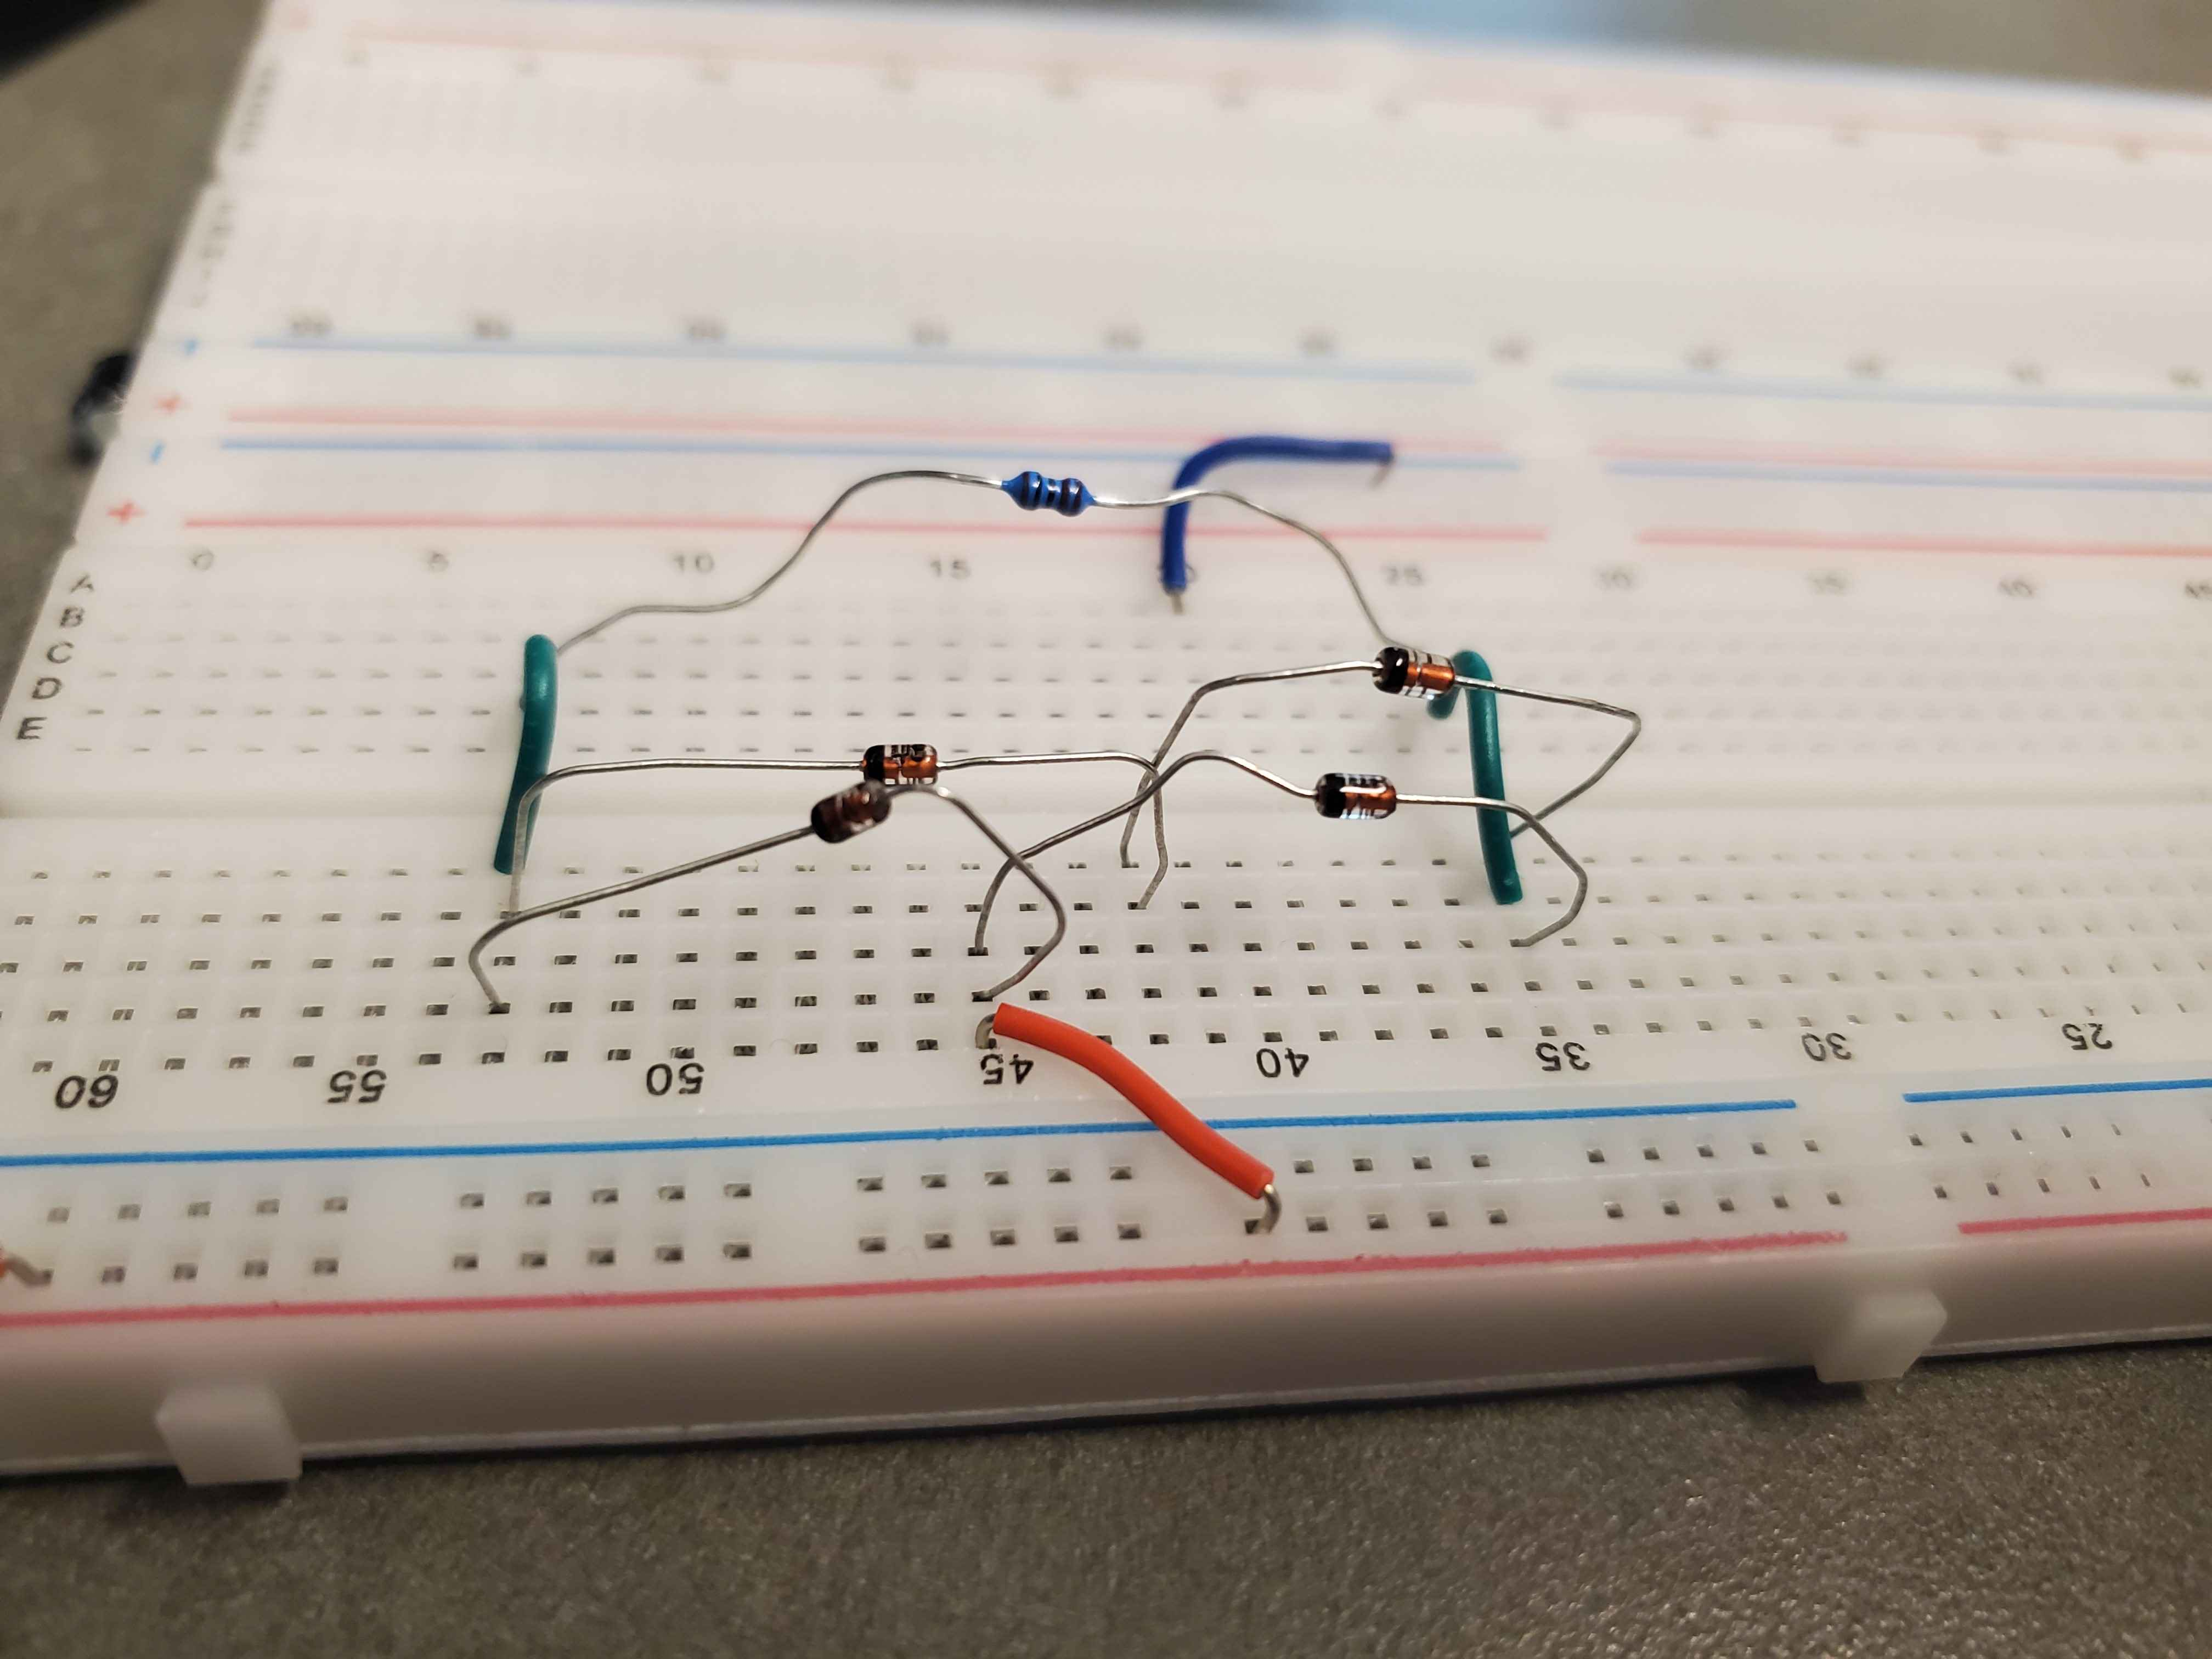
\includegraphics[width=9cm]{20240703_130140}}\hfil
		\subfloat[\centering LTSpice + Rudimentary Schematic Full-Wave Bridge Rectifier with output filter and Zener diode regulator as its output]{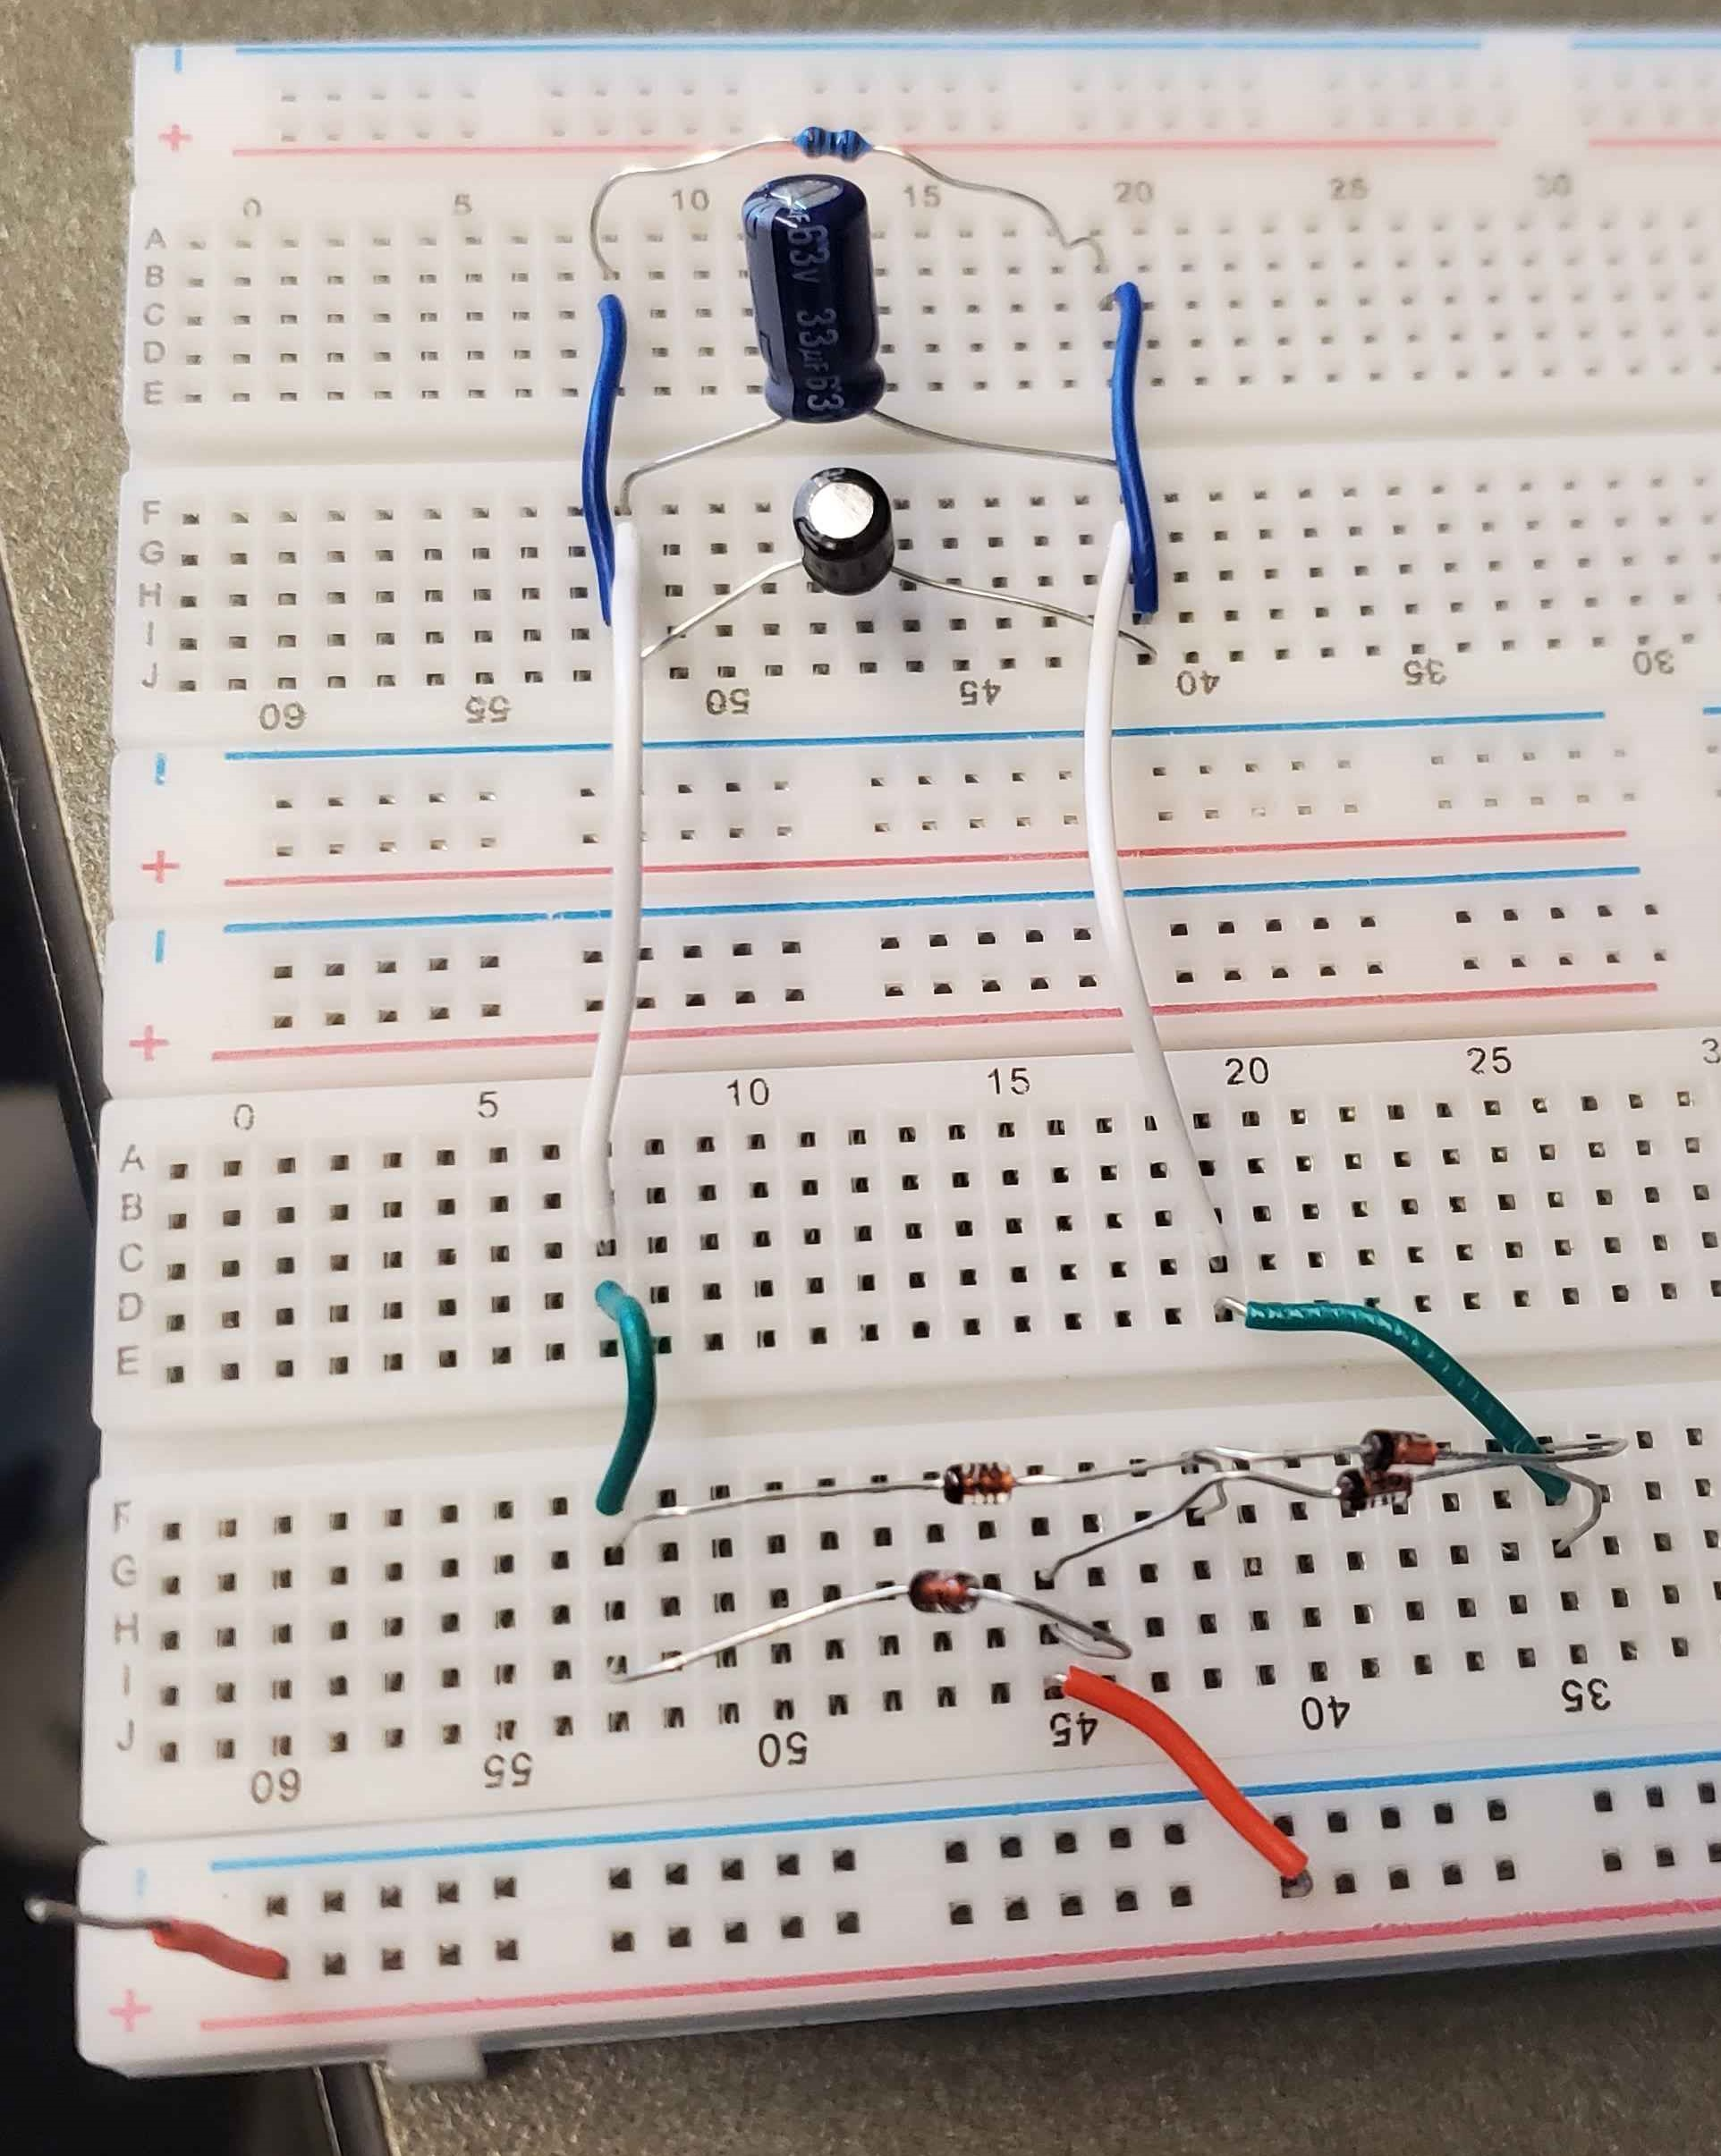
\includegraphics[width=6cm]{20240703_131410}}\hfil
	\end{figure}
	
	\nsection{Descriptions of Measurements \& Calculations}
	Given the default theoretical calculation for a Diode in forward-bias: $I_D=I_S(e^{\frac{V_D}{V_T}}-1)$; the dataset is similar in-nature - not exact because the characteristics of this diode differs - from section 1.1 of the lab.\\
	The characteristic of a \textit{Zener} Diode is its relationship to $-V_D$, as $I_D$ enters \textbf{Reverse-Breakdown} @ $-V_{Z0}$; the point of breakdown.\\
	The utilisation of the Capacitors in the Bridge Circuit is to dissipate the voltage curve over a gentler duration.
	Because of these characteristics, the Bridge Circuit essentially dampens and \emph{Rectifies} the entering voltage; $V_{in}$ to $V_o$
	\begin{figure}[h!]
		\centering
		\caption{Bridge Rectifier Circuits Scope}
		\subfloat[\centering Full-Wave Bridge Rectifier]{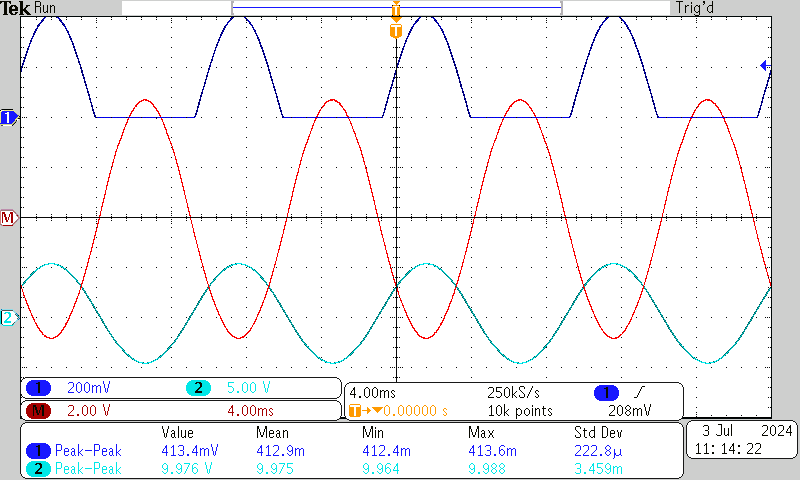
\includegraphics[width=9cm]{tek0000a}}\hfil
		\subfloat[\centering Full-Wave Bridge Rectifier with output filter]{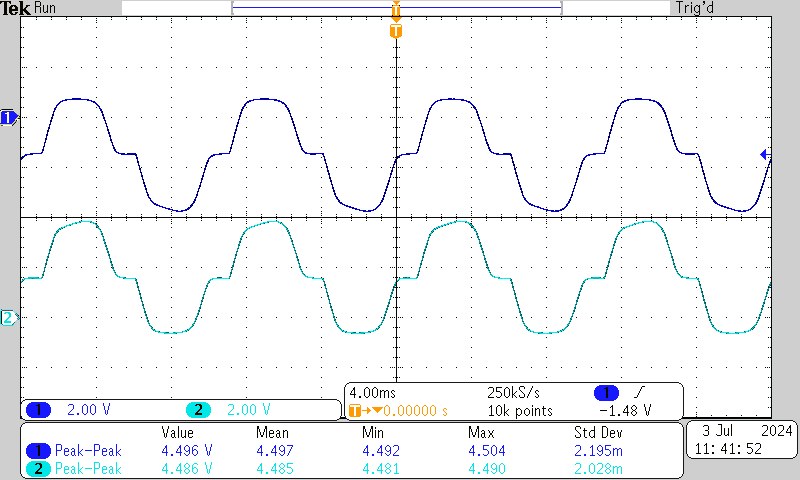
\includegraphics[width=9cm]{tek0001b}}\hfil
		\subfloat[\centering Full-Wave Bridge Rectifier with output filter and Zener diode regulator as its output]{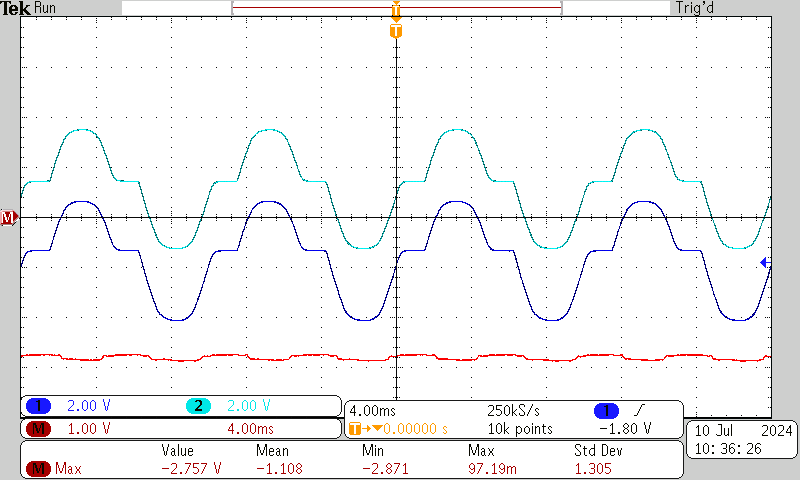
\includegraphics[width=9cm]{tek0001c}}
	\end{figure}
	
	\nsection{Summary \& Conclusions}
	Revealed in Figure RDD-Circuit 0A \& 0B, the generated oscilloscope readings of the two periodic function do in-fact dampen @ $V_{in}$ (CH2) greatly to $V_{out}$ (CH1). It is similary in the Series $D_Z$ circuit.
	\nsubsection{Discussion}
	\begin{itemize}
		\item \textbf{i. Compare the measured versus simulated data and explain any differences.}
		\subitem The measured and simulated data find differences in components, breakdown region, ideal components; which differs in threshold ranges and dampening ranges, and a consistent AC signal that has no attenuation.
		\item \textbf{ii. What are the purposes of experiment 1.41, 1.42, and 1.43? You can explain this by comparing the output voltage waveforms.}
		\subitem The purpose of 1.4.1 is to limit the negative values of the AC waveform. The output voltage had no voltage under 0.
		The purpose of 1.4.2 is to have the circuit charge the capacitors at the turn-on voltage for the diodes then when the input is low enough the capacitor will discharge slowly creating a more linear signal.
		\item \textbf{Is it desirable to reduce the output ripple voltage? Why do you think that is?}
		\subitem Signal alignment; although, we would have to consider using a secondary signal system to propgate the missing values - we'd have a consistently voltage running at a timer rate scaling with total Impedances and Voltage output.
		\subitem It could also be desirable to reduce the output voltage of the ripple because the output voltage might be used for other components that need a certain voltage to operate. So, the ripple voltage can be changed to meet those needs.
		\item \textbf{At what load resistance does the regulated full-wave bridge rectifier come out of regulation?}
		\subitem $R_{Load}\geq1k\Omega$
		\item \textbf{Explain how you would predict the minimum value of the load resistance for which the Zener diode still operates in the breakdown region.}
		\subitem Deriving the theoretical calculation of the Zener Diode's breakdown range; $V_o=V_i-R_i*_i$ @ $D_{Z_{BR}}$, and considering $R_{Load}\geq(R_2*\epsilon)$.
	\end{itemize}

	\newpage
	\nchapter{Addendum Pages}
	\begin{figure}[hp!]
		\centering
		\caption{Jason Truong Addendum}
		\subfloat[\centering Lab Design   Calculations]{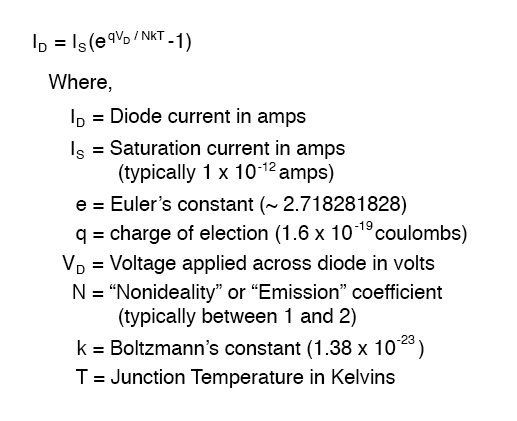
\includegraphics[width=17cm]{Theoretical Calculation of Ideal Diode}}
	\end{figure}
	\newpage
	\nsection{Bibliography}
	\textbf{Cited:}\\
	\begin{itemize}
		\item Lab 1 Manual
		\item Sedra, Adel, and Kenneth Smith. Microelectronic Circuits. S.L., Oxford Univ Press Us, 2019.
		\item “How Do You Calculate, a Silicon Junction Diode with N = 1 Has v = 0.7 v al I = 1 MA. What Is the Voltage Drop at I=0.1 MA and I=10 MA.?” Quora, 2024, appliedmathematics.quora.com/How-to-calculate-A-silicon-junction-diode-with-n-1-has-v-0-7-V-al-I-1-mA-What-is-the-voltage-drop-at-I-0-1-mA-an?top\_ans=223007030. Accessed 15 July 2024.
	\end{itemize}
	\begin{figure}[!h]
		\subfloat[Look at her, she's perfect.]{
\includegraphics[width=\linewidth]{GodILoveFurina}}
	\end{figure}
\end{document}